\documentclass[11pt]{report}
\usepackage[utf8]{inputenc}
\usepackage[french]{babel}
\usepackage[T1]{fontenc}
\usepackage{geometry}
\usepackage{graphicx}
\usepackage{svg}
\usepackage{amsmath}
\usepackage{float}
\usepackage{hyperref}
\usepackage{tikz}
\usepackage{booktabs}
\usepackage{cite}
\usepackage[skip=10pt, indent=20pt]{parskip}

\geometry{
a4paper,
left=1in,
top=1in,
right=1in,
bottom=1in,
}

\newcommand\Chapter[2]{\chapter
  [#1\hfil\hbox{}\protect\linebreak{\itshape#2}]%
  {#1\\[2ex]\large\itshape#2}%
}

\title{Rapport du projet intégré: groupe 2}
\author{Joey Brynckman, Andrea Dal Molin, Thibault Havet, Florent Raeymaeckers,  \\ Arnaud Rase, William Tea, Lionel Thys \& Alexandre Villance}
\date{Q2 2022-2023}

\begin{document}

\maketitle

\tableofcontents

\chapter*{Abstract}

Ce rapport est un descriptif du projet sur lequel nous avons travaillé en tant qu'équipe d'étudiant de la Haute école de la Province de Liège. Nous devions mettre en place un système de paiement sur base d'un énoncé donné durant le mois de Mars 2023. Le but est d'avoir une plateforme qui peut être accédée par un utilisateur qui souhaite effectuer un paiement en ligne vers un marchand.

Notre solution à ce problème regroupe de l'authentification, de l'exploration de données, de la sécurisation de données et du déploiement de serveurs. Nous allons développer ces points ci-dessous.

\chapter{Introduction de l'équipe}

Notre équipe est composée de 8 personnes:

\paragraph{Joey Brynckman} (Serveur marchand, application Android \& bases du National Bank Server)

Je me suis occupé principalement de la partie marchande de notre application. J'ai donc créé le serveur
permettant de contenir les données relatives aux comptes et aux produits à vendre. Pour ce faire, je me
suis donc occupé de la création de la base de données, de l'accès à ses données grâce à un ORM, de l'API
et de la sécurisation de ses endpoints.

Comme le National Bank Server fonctionne sur un principe similaire au serveur marchand, je me suis
donc également occupé de ces aspects de ce serveur. Bien sûr, pour le NBS, il y a beaucoup plus à faire
que ça, notamment l'accès aux bases noSQL et la génération de données, mais c'est Thibault qui s'est
occupé de ces parties-là. Je n'ai fait que la base de ce serveur.

Enfin, je me suis également occupé de l'application Android. Ses pages, leur fonctionnement, ainsi que
les accès à l'API du serveur que j'ai créé. Seule la page de paiement n'a pas été faite par moi, comme il
s'agit d'une page web, d'un portail de paiement créé par Lionel.

Mon choix de faire ces parties vient du fait que j'avais moi-même commencé un projet personnel qui
fonctionnait de manière similaire à notre application Android et notre serveur marchand. J'avais donc
certaines bases et connaissances que j'ai pu utiliser à bon escient.

\paragraph{Andrea Dal Molin} (Responsable Java Card \& beID)

L'intégration de l'authentification via carte d'identité électronique et la gestion des cartes de fidélité ont été mes principales tâches au sein du groupe. Les raisons de ce choix se justifient par la possession personnelle du matériel utile au développement de ces parties, notamment pour ce qui concerne la lecture de carte d'identité électronique. 

De plus, je portais personnellement un intérêt particulier quant à l'intégration de ces deux technologies différentes avec une architecture complète comme celle du Projet Intégré. Comme il sera décrit dans la partie concernant mes sujets, le développement des parties s'est révélé stimulant. 

\paragraph{Thibault Havet}
\paragraph{Flo Raeymaeckers} (DevOps \& Responsable Équipe)

Je me suis occupée de l'infrastructure logicielle du déploiement de la solution. Plus précisément, j'ai mis en place un cluster de serveurs afin que l'ensemble des services que l'on voulait déployer sur le serveur puisse profiter d'un load balancing et d'une virtualisation par container afin d'avoir une scalabilité horizontale des services en fonction de la demande.

De plus, j'ai géré l'équipe. J'ai travaillé sur la mise en commun des ressources (réunions, outils de suivi de projet...), de ce rapport, et enfin de la présentation que vous allez pouvoir assister. Je vais passer en revue dans ce document les différentes difficultés par lesquelles je suis passée et les éventuelles solutions que j'ai apporté.

\paragraph{Arnaud Rase} (Responsable réseau \& aide en DevOps)

Pour ma part, j'ai été mit en charge de l'implémentation de la partie sur le réseau privé de la
banque Picsou. J'ai également aidé Florent à lier celle-ci aux différents serveurs hébergés sur
l'ESXi. L'infrastructure aura 2 grandes parties, la partie routage et switching, nous pourront
notamment retrouver du load balancing, de la traduction d'adresses IP publiques en adresses
IP privée et une disponibilité presque ininterrompue

\paragraph{William Tea}
\paragraph{Lionel Thys}
\paragraph{Alexandre Villance}

\chapter{Étude et mise en théorie de l'infrastructure}

Dans ce chapitre, nous allons passer en revue l'étude que nous avons effectué sur l'énoncé du projet transmit pas nos professeurs. Le projet part d'un énoncé basé sur une version "simplifiée" de 3D secure, ou du moins plus ou moins cousine: nous avons un marchand qui souhaite pouvoir proposer à ses clients la vente de ses services/bien en ligne. Afin que le consommateur puisse payer, le marchand a besoin d'une plateforme de paiement en ligne. Notre rôle est d'implémenter cette plateforme de payement au niveau de la banque du consommateur, qui va alors se synchroniser avec la banque du marchand pour valider la transaction.

\section{Schéma de l'infrastructure}

\part{Implémentation des services}

\Chapter{Déploiement de l'infrastructure}{Arnaud Rase \& Flo Raeymaeckers}

Chaque service que nous mettons en place nécéssite implicitement d'être hébergé quelque part. N'ayant pas les moyens de nous offrir un VPS pour le déploiement de l'intégralité des services sur lesquels nous avons travaillé, nous avons pris l'opportunité de déployer ces derniers sur un serveur mis à disposition pour le projet à l'école.

Ce serveur est une machine HP de type rack 1U qui fait tourner le système d'exploitation ESXi\footnote{OS de gestion de machines virtuelles de VMware}. Grâce à cela, nous pouvons lancer des machines virtuelles sur lesquelles tourneront nos différents systèmes d'exploitation.

Bien évidemment, dans un scénario plus réaliste, nous n'aurions pas seulement un serveur, mais plusieurs. Les ressources de l'école nous limite à n'utiliser qu'un serveur physique. Nous considèrerons alors que chaque système d'exploitation tournant sur ESXi soit en fait un serveur physique qui va, plus tard, faire partie d'un "cluster". Je vais revenir sur ce terme là un peu plus tard.

\section{Virtualisation des services}

\begin{figure}[H]
    \centering
    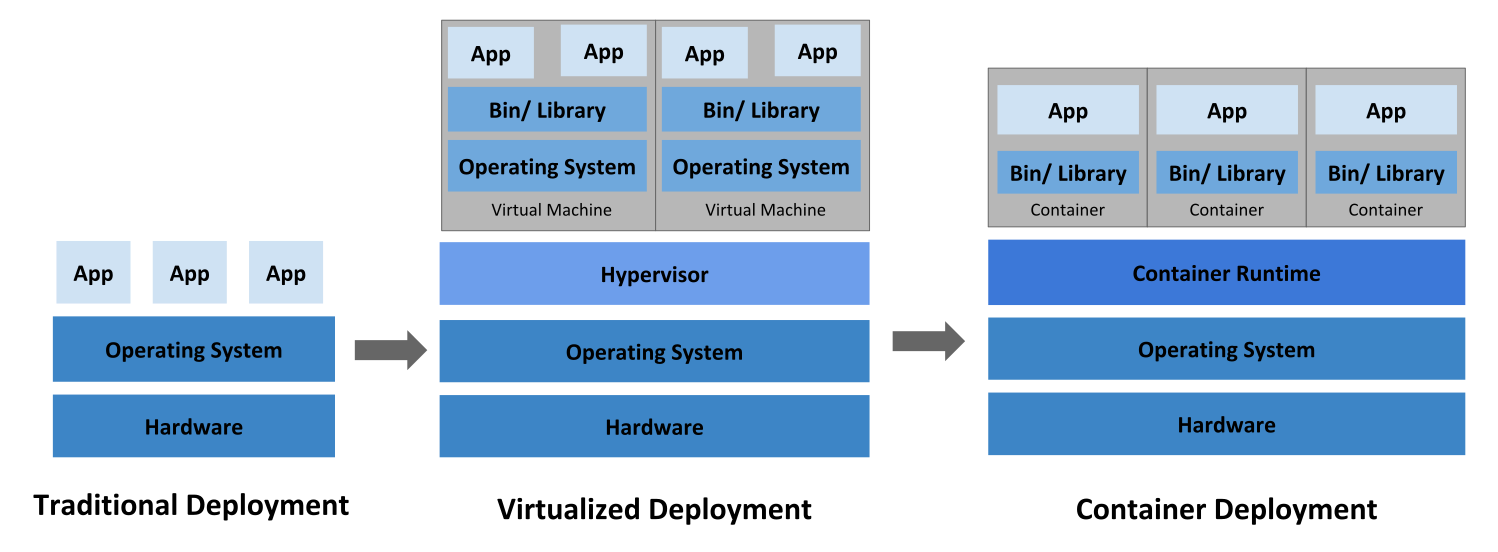
\includegraphics[width=\textwidth]{./img/container_evolution.png}
    \caption{Évolution du déploiement d'applications \cite{shavidissa2019}}
    \label{fig:container_evolution}
\end{figure}

Traditionnellement, lorsqu'une application devait être déployée et rendue utile au grand public, elle était simplement exécutée sur le système d'exploitation de la machine physique hôte. Ce "déploiement traditionnel", qui, à la surface, semblait simple, posait en fait, au long terme, bien des problèmes. On peut citer des problèmes de sécurité car l'application cohabiterai avec d'autres applications ou bien des problèmes de scalabilité, où les applications sont limités au niveau des ressources qu'offre le hardware de la machine, mais aussi des problèmes où l'application dépendrait de l'intégrité du système dans lequel elle est installée.

Pour palier à tout ça, une des solutions est de travailler avec des machines virtuelles. Un hyperviseur va pouvoir orchestrer différents systèmes d'exploitation dans lesquels résideront les services que nous souhaitons déployer. Ainsi, chaque service sera isolé des autres. De plus, il est possible de mettre en place un système qui, en cas de défaut d'une instance d'un service ou en cas de demande saturée du service, il est possible de lancer, à la volée, une machine virtuelle qui ferait tourner ce service. Rendant ainsi possible un load balancing des requêtes envers ce service. Un des seuls soucis avec tout ça, c'est que l'utilisation des machines virtuelles présente un overhead plutôt conséquent.

La solution que nous avons opté découle des deux solutions ci-dessus. Elle améliore le service en le redant:

\begin{itemize}
    \item plus isolé
    \item plus facilement instanciable
    \item moins coûteux en terme d'overhead
\end{itemize}

Le principe est d'avoir plusieures machines présentant chacune leur propre système d'exploitation (ici, Linux\footnote{ou plus précisément, Ubuntu 23.04}). Dans ces systèmes d'exploitation tourneront des moteurs de containerization, comme Docker.

\subsection{Docker}

Comme dit précédemment, La technologie de containerization que nous allons utiliser s'appelle Docker. Elle permet de "construire" notre propre container avec le service que nous souhaitons déployer. Il restera alors à dire à Docker de déployer un service untel et le service se déploiera\dots N'est-ce pas ?

Certains d'entre vous me diront "Mais Flo, qu'en est-il de l'orchestration des différents services, tu sais, l'avantage que nous présentais le deuxième point ?". Malheureusement, jeune padawan, Docker ne nous permets pas ça. Il permet d'isoler un environnemnt mais sur qu'une seule machine. Travailler en harmonie avec d'autres moteurs docker reste impossible\dots ou du moins sans notre dernière solution.

\section{Kubernetes}

Kubernetes fait partie de la famille des orchestrateur de containers. C'est une couche au dessus qui va s'occuper de lancer  des pods\footnote{l'unité la plus petite de kubernetes. Elle comprend un ou plusieurs containeurs qui travaillent ensemble} dans un cluster\footnote{un groupe} de nodes\footnote{les serveurs sur lesquels vont tourner les containers}.

Notre but étant que, à la place d'avoir une structure verticale de plusieures machines qui s'occuperont de nos services, nous avons opté sur une structure horizontale. Le principal est que, depuis un entrypoint singulier (ici, l'ingress), on peut accéder plusieurs différents services.

\subsection{Administration du cluster}

L'administration du cluster est une épreuve assez fastidieuse. Je vais décrire ici les différents aspects de la gestion de cluster:

\paragraph{Initialisation du cluster:} pour cette étape, il faut lancer la commande kubeadm init sur le serveur qui agira comme master. Il faut ensuite spécifier plusieurs paramètres:
\begin{itemize}
    \item \mintinline{shell}|--apiserver-advertise-address| étant donné que je travaille sur un serveur avec plusieurs interfaces réseaux (une interface pour la connexion entre les nodes et une interface qui fait connexion temporaire internet), j'ai dû préciser l'adresse IP sur laquelle on écoute les appels vers l'API Kubernetes\footnote{l'API est le moyen principal pour que les nodes communiquent entre-eux. Ils communiques par HTTP et l'API se situe sur le master-node}. En l'occurence, j'y ai mis l'IP 172.16.100.18/29.
    \item \mintinline{shell}|--cri-socket| étant donné que Kubernetes est totalement indépendant de gestionnaire de containers, il faut pouvoir spécifier un CRI, c'est-à-dire un Container Runtime Interface.\footnote{vous l'aurez compris, nous avons choisi Docker pour remplir ce rôle}
    \item \mintinline{shell}|--pod-network-cidr| nous ne l'avons pas utilisé, mais il est important de spécifier que ce dernier permet de spécifier un network virtuel sur lesquels vont communiquer les pods. Il est indifférent des networks physiques que nous avons mis en place.
\end{itemize}
L'initialisation du cluster finie, il faut ensuite pouvoir joindre les worker nodes avec la commande kubeadm join, prenant en paramètre l'adresse IP du master node.

\paragraph{Container Network Interface plugin:} un inconvéniant et un avantage de kubernetes est l'utilisation obligatoire d'un plugin d'interface réseau. Aux premiers abords, j'ai trouvé ça perturbant, surtout sur "comment choisir le bon plugin ?". Ayant creusé un peu, j'ai finalement pu prendre le plugin Flannel, qui est plus ou moins populaire. Cependant, il est intéressant de noter que certains plugins peuvent prendre en compte le protocol BGP ou peut permettre bien d'autres choses. Je ne vais pas rentrer dans les détails cependant. Le déploiement du plugin se fait sur le node master et se répliquera dans les nodes workers automatiquement.

\paragraph{Container Storage Interface:} le dernier obstacle qui me barrait la route au bon fonctionnement d'un déploiement d'un pod sur le cluster était la mise en place d'un système de stockage. Le principe du système de stockage dans Kubernetes est de créer ce qu'on appelle des "Persistant Volume". Après la création desdits storages, un pod va demander une certaine taille de stockage avec un "Persistant Volume Claim". Nous avons choisi la façon la plus basique de stocker des données, c'est à dire sous un dossier dans une VM. Mais il est cependant possible de le faire avec du iSCSI, avec vSphere, GKE, AWS etc.

\paragraph{Serveur de Certificat Authoritaire:} afin de permettre une connexion sécurisée entre un client et les service que l'on met en place, il nous faut un certificat authoritaire qui va s'occuper des différents services. Mieux encore, nous avons opté sur un serveur qui accepte le protocol ACME, ainsi, il sera possible d'automatiser le renouvellement de certificats grâce au service suivant.

\paragraph{Ingress Nginx:} ceci n'est pas réellement obligatoire au fonctionnement du déploiement, mais j'ai préféré l'utiliser. C'est un plugin qui va faire office de reverse proxy. C'est-à-dire qu'en fonction de l'addresse DNS rensegnée dans la requête, le reverse proxy va rediriger la requête vers le bon service. 

Pour exposer l'ensemble des services sur l'externe, j'ai choisi d'utiliser un NodePort. Avec un NodePort, on va assigner un service (ici, le ingress nginx) sur un port spécifique. Ainsi, le service nginx va être constamment accessible via n'importe quele addresse IP d'un node et le port spécifié dans la configuration d'un NodePort.

\begin{figure}[H]
    \centering
    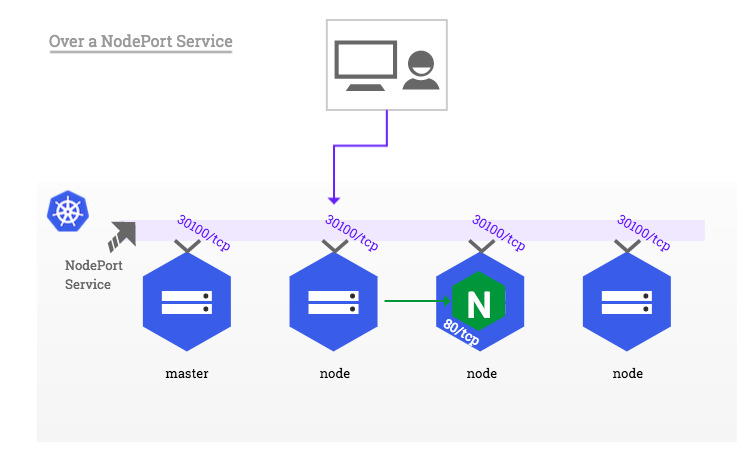
\includegraphics[width=\textwidth]{./img/nodeport.jpg}
    \caption{Représentation graphique d'un NodePort}
    \label{fig:node_port}
\end{figure}

\subsection{Mise en place du déploiement}

Chaque service que nous avons développé/travaillé dessus va se voir être hébergé sur le cluster. Nous avons créé certains containers grâce à des Dockerfiles, tandis que certains autres services fonctionne via docker compose. Heureusement pour nous, Kubernetes a un outils qui s'appelle "Konvert" et permet de convertir un docker-compose en pods kubernetes.

\section{Outil de build et système de contrôle de version}

\subsection{Git \& le contrôle de version}

Git, outil bien connu de tout développeur, a été la principale façon pour nous de partager notre code. Nous avons mis en commun notre code sur la plateforme GitHub, sous une organisation créée pour l'occasion. Chacun allait pouvoir créer un repository pour chaque projet qu'il comptait ajouter à la solution finale. De plus, github nous permet de gérer un repository d'images Docker et de librairies Maven qui nous permettra, in fine, de les téléverser dessus.

\subsection{Gradle, l'outil de build logiciel}

Comme la majorité des personnes de notre groupe souhaitait travailler avec le JVM, j'ai voulu mettre en place un moyen pour eux de simplement entrer le plugin correspondant à leur type de projet dans leur gradle, et ainsi ils n'avaient qu'à coder. Ils ne devaient pas se soucier de "comment déployer l'application".

Il y avait trois types d'applications:

\begin{itemize}
    \item L'application finale: c'est-à-dire une application lancée par un utilisateur final. Cette dernière peut-être l'application mobile ou bien l'application desktop de lecture de carte d'identité. Ces applications ne nécessitaient pas réellement de déploiement à proprement parlé.
    \item L'application serveur: ce type d'application va être héberger sur un serveur. Dans notre cas, ça sera dans le cluster Kubernetes mis en place précédemment. Le principal est alors de placer tout ça dans un container docker. Jib, un plugin gradle spécialiser dans la containerization de services du JVM, a été le plugin de choix pour créer un docker et pour pouvoir le téléverser sur GitHub Packages.
    \item L'application librairie: \footnote{résultante d'un abus de language, une application n'est pas forcément une librairie} ces dernières sont similaire aux containers Docker, à la différence qu'elle seront hébergées sur un serveur Maven, aussi offert par Github.
\end{itemize}


\Chapter{Mise en place de la topologie réseau}{Arnaud Rase}

\section{Topologie Réseau}

\begin{figure}[H]
    \centering
    \includegraphics[width=\textwidth]{./img/Projet réseau.png}
    \caption{Topologie du réseau}
    \label{fig:arnaud-topo}
\end{figure}

Pour la partie routage du réseau, le protocole BGP a été mis en place afin de communiquer
entre les différents ISPs et systèmes autonomes (AS). L'utilisation de 2 ISPs différent permet
l'accès à internet et la connectivité avec d'autres réseaux externes. BGP quant à lui prend en
charge le routage dans un environnement où plusieurs AS interagissent. La double relation
entre les routeurs R2 et R3 sont de l'IBGP alors que celles entre les ISPs, l'internet et les
routeurs 2 et 3 sont de type EBGP. Afin de faciliter la communication entre les différents liens,
l'interface de loopback a été utilisée pour donner une interface de « référence » virtuelle qui
ne changera pour s'occuper de ces communications. Il a également été imposé que les deux
ISPs ne puissent pas communiquer entre eux via le réseau privé, celui-ci ne doit pas servir de
zone de transit.

Une fois rentré dans la partie « privée » du réseau, c'est le protocole EIGRP qui prend le relai
afin de rediriger les paquets venant de l'internet vers routeur 1 qui aura la charge de PAT/NAT.
Contrairement au BGP utilisé pour communiquer entre plusieurs AS, EIGRP se concentre sur
le routage au sein d'un même AS. Une fois la traduction terminée, R1 va pouvoir amener les
paquets vers le serveur qui sera utilisé.

Pour accéder au serveur, le paquet passera par une partie switchée qui a le spanning-tree
protocol de configuré. Celui-ci permet d'empêcher les boucles potentielles tout en conservant
une certaine redondance. Avec cela les potentiels problèmes de congestions liés aux boucles
n'auront pas lieu.

L'utilisation conjointe de VLAN et de HSRP permet de gérer d'une façon plus fluide et plus
adaptée les différentes requêtes de chaque serveur.

Le VLAN permet d'avoir une sécurité améliorée en segmentant le réseau en groupes logiques
distincts. Cette segmentation profite également au niveau des performances en répartissant
les charges pour une meilleure gestion des ressources.

Le HSRP permet lui une meilleure disponibilité du réseau d'une façon un peu similaire au
spanning-tree. L'utilisation simultanée de ces deux protocoles permet une gestion efficace des
ressources, une redondance et un rétablissement automatique.

Dans le cadre de ce projet, il a été convenu d'utiliser la version d'essai de Cisco Modeling Labs.
Malheureusement celle-ci ne vient pas sans restriction, la connexion au réseau externe via un
« external connector » ne fonctionne pas empêchant d'intégrer la topologie montrée
précédemment au reste du projet. Le « switch virtuel » présent dans la topologie est là pour
représenter à quoi aurait dû ressembler la topologie si la connexion avait été possible.


\Chapter{Configuration d'un service d'authentification centralisé}{Lionel Thys}

Pour l'authentification du client au niveau de sa banque, nous avons opté pour une implémentation
externe d'un service d'authentification. De ce fait, nous séparons bien le développement de
l'application de la banque et son authentification.
L'authentification du client est une fonctionnalité primordiale pour le fonctionnement de l'ACS.

\section{Keycloak}

\begin{figure}[H]
    \centering
    
\includegraphics[scale=.1]{./img/Keycloak.png}
    \caption{Icône du logiciel Keycloak}
    \label{fig:keycloak_logo}
\end{figure}

Keycloak est un software d'authentification open-source
possédant une grande communauté. Ce software est
utilisé pour l'authentification de plusieurs entreprises à
travers le monde, ce qui nous rapproche d'une
infrastructure réelle. Nous l'avons choisi pour:

\begin{itemize}
    \item Séparer la partie fonctionnelle de l'ACS et
    l'authentification du client
    \item Créer une plateforme d'authentification la plus
    fidèle possible à la réalité
    \item Apprendre de nouvelles technologies
\end{itemize}

Keycloak possède plusieurs fonctionnalités appréciables à la création du projet. Notamment le
déploiement via Kubernetes ou Docker.

\subsubsection{Single-Sign On (SSO)}

Keycloak implémente la fonction de SSO : le client n'a besoin de s'authentifier qu'une seule fois et
sera automatiquement connecté si le token créé à la première connexion est toujours valide.

\subsubsection{Connexion à des base de données existantes}

Keycloak peut se connecter à une base de données relationnelle existante, mais aussi un serveur
Active Directory ou LDAP. Cela permet de créer plusieurs instances de keycloak connecté à la même
base de données.

\begin{figure}[H]
    \centering
    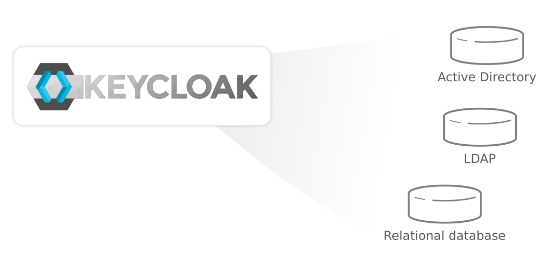
\includegraphics[width=\textwidth]{./img/Keycloak-Existant-Data.png}
    \caption{Différentes sources de données peuvent être configurées pour Keycloak}
    \label{fig:keycloak_data_source}
\end{figure}

\subsubsection{Identity Providers}

Keycloak prend le rôle d'Identity Provider via les protocoles OpenID Connect (OIDC), OAuth 2.0 ou
SAML 2.0. Cela nous permet de nous connecter en utilisant des librairies implémentant ces deux
protocoles. Pour l'application web de la banque, faite en React, nous avons utilisé la librairie react-
oidc d'AXA (le groupe d'assurance).

Mais ce n'est pas tout. Grâce à cette implémentation, nous pouvons aussi nous identifier par des
Identity Provider existant, tel que Google, Github, Facebook, \dots

\begin{figure}[H]
    \centering
    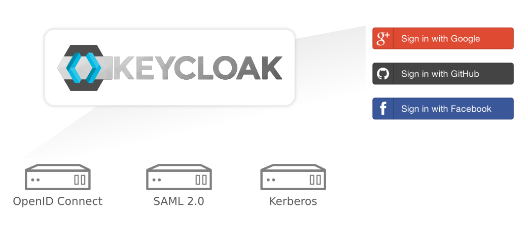
\includegraphics[width=\textwidth]{./img/Keycloak-Identity-Provider.png}
    \caption{Keycloak et ses différents IDP}
    \label{fig:keycloak_idp}
\end{figure}

\subsection{Fonctionnement}

\subsubsection{Realms}

Keycloak intègre la notion de royaumes, ou realms qui implémente chacun leur client de connexion,
leurs utilisateurs, leurs serveurs SMTP, ... Ces realms permettent par exemple de créer une
infrastructure par site pour une entreprise possédants plusieurs sites.

Prenons l'exemple de l'entreprise John Cockerill. En implémentant un realm pour le site de Seraing et
un autre pour le site de Loncin, les administrateurs du site de Seraing ne peuvent pas interagir sur le
site de Loncin.

Bien évidemment, il y a un realm master, permettant d'interagir en tant qu'administrateur. Ce realm
est unique et est le seul permettant d'interagir sur les autres realms.

\begin{figure}[H]
    \centering
    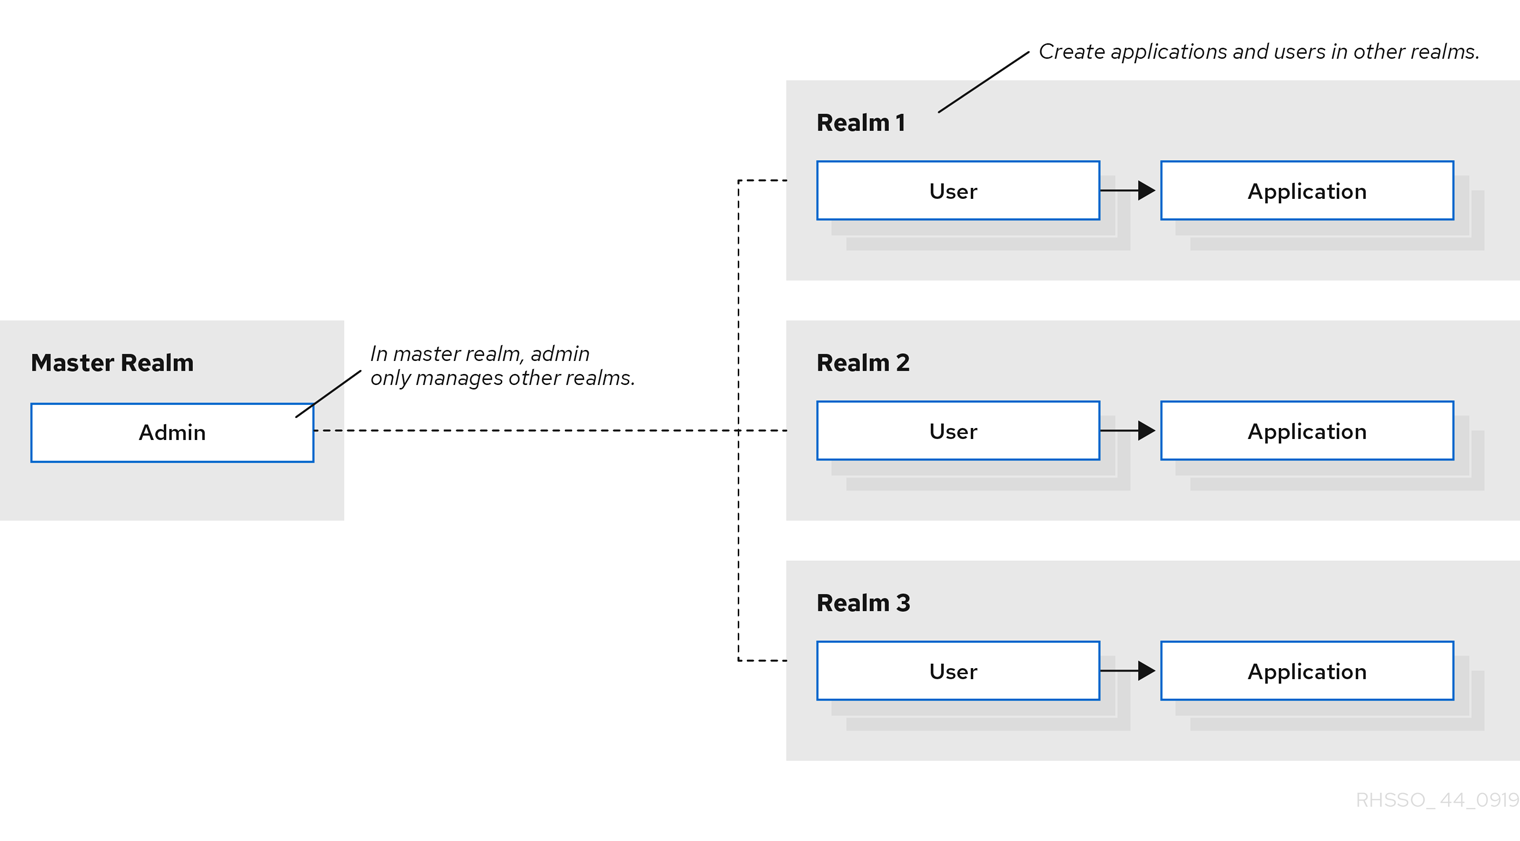
\includegraphics[width=\textwidth]{./img/Keycloak-realm.png}
    \caption{Les Realms ou "Royaumes" de Keycloak}
    \label{fig:keycloak_realms}
\end{figure}

\subsubsection{Clients}

Les clients représentent les moyens de connexion disponible sur le realm. Ces clients possèdent
plusieurs paramètres :

\paragraph{Root URL:} l'url qui servira à accéder au client

\paragraph{Valid Redirect URIs:} Ce sont les urls de redirections autorisées lors de la connexion. Si l'on désire
accéder à une ressource via une url non autorisée, le client nous en empêchera. Nous pouvons en
mettre plusieurs.

\paragraph{Valid post logout redirect URIs:} Pratiquement la même chose que les redirect URI, sauf qu'ici, cela
n'est valide que pour les opérations de logout.

\paragraph{Web Origins:} Ce sont les urls autorisées à accéder au client. Cela est surtout utile lorsque l'on se
connecte à un super-utilisateur, pour éviter les connexions externes au réseau de l'entreprise. On
évite alors les connexions frauduleuses.

\paragraph{Login Theme:} C'est le choix du style du formulaire de connexion.

\paragraph{Browser Flow:} Le formulaire d'authentification est défini par realm, mais nous pouvons forcer un
formulaire spécifique par client.

\subsubsection{Users}

Les utilisateurs sont soit créé sur une page d'enregistrement prévue à cet effet, soit créé via un super-
utilisateur. Pour des raisons de sécurité et d'approche plus réaliste, nous avons choisi la création via
super-utilisateur.

Lors de la création, deux valeurs sont obligatoires : l'id (généré automatiquement) et l'username (que
l'utilisateur encode). Nous pouvons ajouter un prénom et un nom ainsi qu'une adresse mail. Cette
adresse peut servir de remplacement au nom d'utilisateur.

Nous pouvons aussi forcer des actions à l'utilisateur qu'il devra effectuer à sa prochaine connexion tel
que:

\begin{itemize}
    \item La configuration du gestionnaire d'OTP (Google Authenticator,...)
    \item La modification du mot de passe.
    \item \dots
\end{itemize}

Nous pouvons aussi ajouter des credentials (i.e. password), que nous implémenterons via les actions définies juste
avant.

Et enfin, nous pouvons ajouter des attributs à l'utilisateur, tel que:

\begin{itemize}
    \item Le numéro de téléphone (mobile-number) utilisé pour la connexion SMS.
    \item Le genre
    \item La date de naissance
    \item \dots
\end{itemize}

Nous avons aussi les informations de sessions active de l'utilisateur, mais nous pouvons avoir ces
données pour l'ensemble des utilisateurs du realm via l'onglet Session.

\subsubsection{Events}

Les events sont avant tout des informations de log. Ces informations peuvent être exploitée pour des
informations de connexions (adresse ip, le client, l'utilisateur, le royaume, la date de l'event, ...). Ces
events ont un type (LOGIN, LOGIN-ERROR, LOGOUT, REDIRECT-TOKEN, ...) ce qui nous permet de
savoir les actions de l'utilisateur (directes ou indirectes).

\subsubsection{Authentication Flow}

Ces flux d'authentification représentent les différents formulaires d'authentifications discutés dans la
partie Clients. Nous pouvons choisir les conditions de connexion tel que via cookie (pour le SSO), via
Identity Provider (pour une connexion via Google, ...) ou encore via un formulaire customisé.

\subsubsection{Providers externes}

Keycloak supporte l'ajout de librairies externes. Nous en avons utilisé et créé pour:

\begin{itemize}
    \item La connexion 2FA via SMS
    \item La connexion 2FA via Mail
    \item La sauvegarde d'event customisée pour stockage sur une BD MongoDB
\end{itemize}

Pour se faire, nous devons juste inclure le(s) fichier(s) .jar dans l'onglet provider du serveur de
Keycloak.

Dépendant de la librairie, nous avons des parties de formulaire (pour l'authentification 2FA) ou des
EventListener à lier aux events du realm.


\Chapter{Création d'une application marchande PoC}{Joey Brynckman}




\Chapter{Mise en place d'une cellule d'analyse de données}{Thibault Havet}

\section{Vue globale}

\begin{figure}[H]
    \centering
    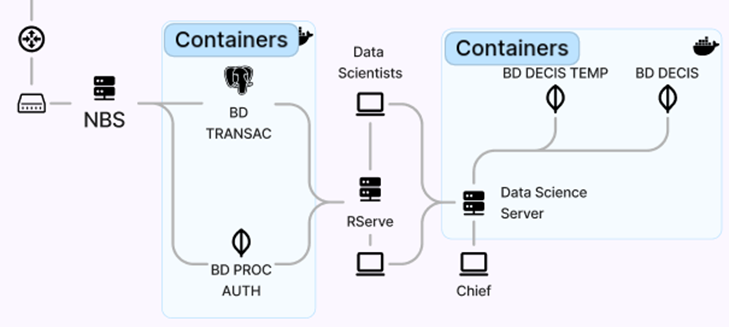
\includegraphics[width=\textwidth]{./img/thibault-VueGlobale.png}
    \caption{Vue globale du projet}
    \label{fig:thibault-global-view}
\end{figure}

\section{Data scientist application}

Cette application a été programmée en Java, développé avec le JDK17 et est gérée grâce à Gradle. Elle
utilise les frameworks suivants:

\begin{itemize}
    \item JavaFX afin de créer les interfaces graphiques. Utilisation du patron de conception Model-View-ViewModel.
    \item Spring boot afin de pratiquer l'injection de dépendance, et d'utiliser un fichier de properties pour configurer l'application sans avoir à la recompiler.
    \item Les librairies REngine et RServe afin de communiquer avec le serveur Rserve.
\end{itemize}

Afin de subvenir aux besoins du data scientist, cette application propose de travailler sur les bases de
données DB\_OPER\_PROC\_AUTH (MongoDB) et DB\_OPER\_TRANSACTIONS (PostGres) via RServe. C'est
le rôle du serveur RServe de récupérer les données dans les DBs et le les proposer au data scientist via
l'application.

De plus, cette application offre la possibilité de récupérer les résultats des opérations effectuées sur le
serveur Rserve, et de les manipuler au moyen de plusieurs interfaces JavaFX. Elle implémente les 3
méthodes d'exploration nde données suivantes :

\begin{itemize}
    \item Analyse de composantes principales
    \item Régression-corrélation multiple
    \item ACM
\end{itemize}

Une fois satisfait de l'étude des données, le data scientist peut tirer une conclusion l'envoyer au Data
Science Server via une socket utilisant TLS. Ce dernier les insère alors dans la base de données
DB\_DECIS\_TEMP.

\begin{figure}[H]
    \centering
    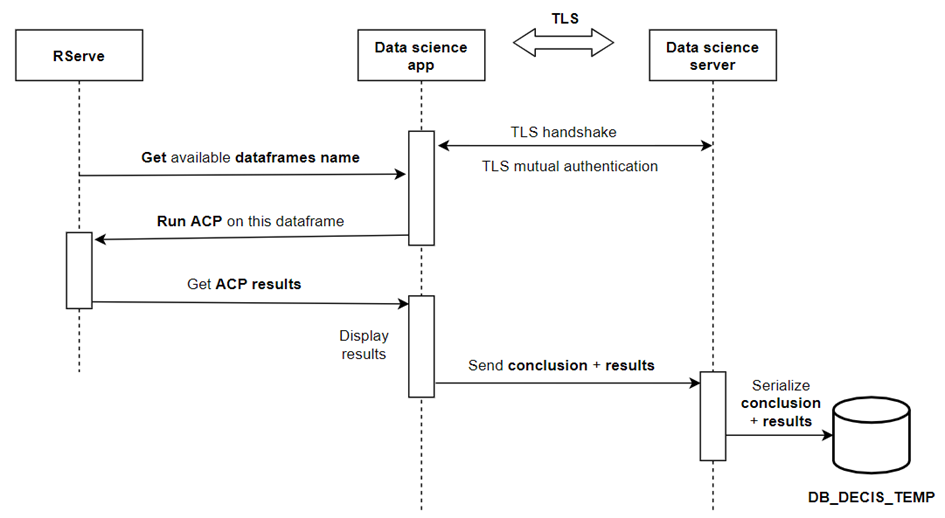
\includegraphics[width=\textwidth]{./img/thibault-DataScientistApp_1.png}
    \caption{Vue globale du projet}
    \label{fig:thibault-rserve-exchange}
\end{figure}

\section{Data Science Server}

C'est lui qui s'occupe de gérer les requêtes des data-scientist et du chief data-scientist. Pour ce faire, le
les requêtes sont gérées par un pool de thread, elles sont mises en attente dans une file en attendant
d'être exécutée par le pool.
Ce serveur est également chargé de sérialiser/désérialiser les conclusions dans les bases de données
DB\_DECIS\_TEMP et DB\_DECIS. Les accès concurrents sont pris en compte (un objet gérant les accès
aux DBs avec des méthodes 'synchronized').
Le type de requêtes autorisées vers ce serveur dépend du certificat du client (en fonction du Designated
Name plus précisément). Un chief data-scientist n'aura pas les mêmes droits qu'un data-scientist, et
n'importe qui ne peut se connecter au serveur et ce, grâce à l'authentification mutuelle de la couche
de sécurité TLS (le client doit lui aussi posséder un certificat, et le Data Science Server doit connaitre le
DN de ce certificat). Pour les plus curieux, s'en référer aux classes suivantes du projet 'data-minings-
apps' :

\begin{itemize}
    \item be.masi.g2.DataScientistServer.Tasks.TaskInstantiation
    \item be.masi.g2.DataScientistServer.ThreadPool.DataScientistServerThread
\end{itemize}

\section{Chief data scientist application}

Tout comme l'application des data scientist, ce logiciel utilise JavaFX, Spring boot ainsi que RServe et
REngine. L'application utilise également une socket utilisant TLS pour communiquer avec le Data
Science Server.
Elle passe par l'intermédiaire du Data Science Server afin de valider ou d'annuler les conclusions
stockées dans la base de données DB\_DECIS\_TEMP.

Récupération des conclusions :

\begin{figure}[H]
    \centering
    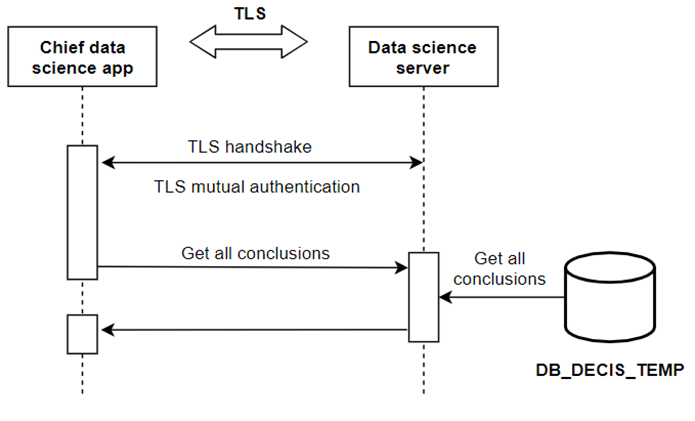
\includegraphics[width=\textwidth]{./img/thibault-DataScientistApp_2.png}
    \caption{Vue globale du projet}
    \label{fig:thibault-chief-app-retrieve}
\end{figure}

Validation d'une conclusion :

\begin{figure}[H]
    \centering
    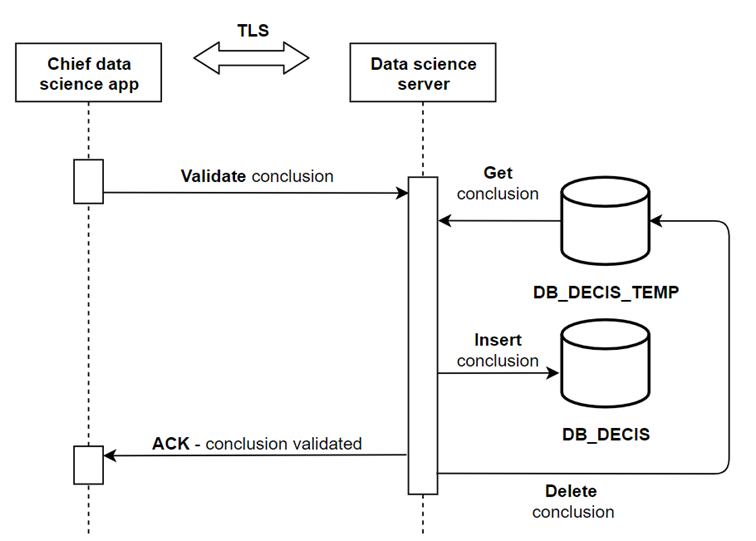
\includegraphics[width=\textwidth]{./img/thibault-DataScientistApp_3.png}
    \caption{Vue globale du projet}
    \label{fig:thibault-chief-app-validate}
\end{figure}

Annulation d'une conclusion :

\begin{figure}[H]
    \centering
    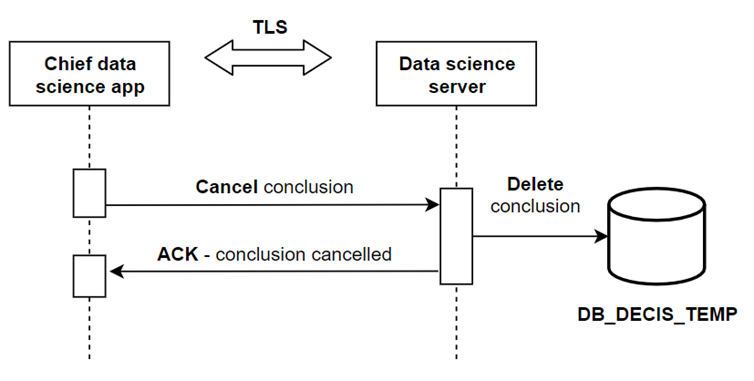
\includegraphics[width=\textwidth]{./img/thibault-DataScientistApp_4.png}
    \caption{Vue globale du projet}
    \label{fig:thibault-chief-app-cancel}
\end{figure}

\section{Serveur RServe}

Serveur prenant en compte les requêtes des data-scientist et du chef des data-scientist (via leurs apps respectives). Il est chargé de récupérer les données des bases de données \\ DB\_OPER\_PROC\_AUTH (MongoDB) et DB\_OPER\_TRANSACTIONS (PostGres) et de les convertir en dataframes exploitables par les data-scientist. De fait, les données contenues dans les bases de données ne sont pas utilisables par le framework 'FactoMineR' (package R consacré à l'exploration de donnée).

Ce script porte le nom de 'ConvertAuthenticationToDataFrame.R' et est disponible dans l'archive jointe.

\subsection{Exemple de traitement des données}

On commence tout d'abord par récupérer les données dans l'une des bases de données. En l'occurrence, la DB\_OPER\_PROC\_AUTH (MongoDB) :

\begin{listing}[H]
    \begin{minted}{r}
library(mongolite)

connection_string = 'mongodb://127.0.0.1:27017'
clientsCollection = mongo(collection="clients", db="DB_OPER_PROC_AUTH", url=connection_string)
clients <- clientsCollection$find()

clientDf <- as.data.frame(clients)
    \end{minted}
    \caption{Récupération des données depuis la DB MongoDB}
    \label{listing:thibault-retrieve-data}
\end{listing}

En l'état des choses, la dataframe clientDf possède la même structure que la collection 'clients' de la
base de données. On a ici récupéré la liste des clients. Chaque document est structuré comme suit :

\begin{listing}[H]
    \begin{minted}{r}
- Clients :
    - Date naissance
    - Sexe
    - Banques
        - Nom
    - OTPs:
        - Date-heure demande
        - âge du client au moment de la demande (automatique)
        - compteur essai
        - temps authentification (date-heure reception - date-heure demande)
        - décision
        - nouvel essai nécessaire ?
        - nombre d'essais dépassé ?
    - SMSs :
        - Data-heure demande
        - âge du client au moment de la demande (automatique)
        - envoi par réseau ou par SMS ?
        - temps authentification (date-heure réception - date-heure demande)
        - hors délai ?
        - décision
    - E-mails :
        - date-heure demande
        - âge du client au moment de la demande (automatique)
        - montant transaction envisagée
        - HTTP ou HTTPs
        - temps authentification (date-heure reception - date-heure demande)
        - hors délai ?
        - décision
    - EIDs :
        - date-heure demande
        - âge du client au moment de la demande (automatique)
        - temps authentification (date-heure reception - date-heure demande)
        - décision
    \end{minted}
    \caption{Structure des données du document}
    \label{listing:thibault-structure-db}
\end{listing}

La structure de cette base de données reste à améliorer. De fait, un document client stocke toute ses
authentifications. Nous sommes conscients qu'il y a un petit problème d'optimisation de place
(certaines données sont dupliquées) et que cela risque également de coincer sur le long terme au
niveau de la taille maximale d'un document sur MongoDB (16Mo maximum par document). Il aurait
fallu créer une collection par type d'authentification. Malheureusement, ayant trop peu d'expérience
en NoSQL, et s'étant rendu compte de l'erreur trop tard (toute l'infrastructure a déjà été construite
autour de cette BD), nous n'avons pas eu le temps de rectifier cela.

Mais revenons-en au traitement de la dataframeclientDf. Pour notre exemple, nous allons créer une
dataframe exploitable par R qui possède les colonnes suivantes : NbreBanque - Genre Age - NbrEID -
NbrEmail - NbrOTP – NbrSMS.

\begin{listing}[H]
    \begin{minted}{r}
nbrAuthDf = data.frame()

clientNbr = nrow(clientDf)

for(i in 1:clientNbr){
    client = clientDf[i,]
    bankNbr = nrow(client$banks[[1]])
    gender = client$gender
    age = as.integer(as.numeric((Sys.time() - client$birthday))/365.25)
    eidAuthNbr = nrow(client$eidAuthentication[[1]])
    otpAuthNbr = nrow(client$otpAuthentication[[1]])
    smsAuthNbr = nrow(client$smsAuthentication[[1]])
    mailAuthNbr = nrow(client$mailAuthentications[[1]])
    nbrAuthDf <- rbind(nbrAuthDf, list(bankNbr, gender, age, eidAuthNbr, mailAuthNbr, otpAuthNbr, smsAuthNbr))
}
colnames(nbrAuthDf) <- c("BankNbr", "Gender", "Age", "EIDAuthNbr", "MailAuthNbr", "OTPAuthNbr", "SMSAuthNbr")
    \end{minted}
    \caption{Récupération des données depuis la DB MongoDB}
    \label{listing:thibault-r-code}
\end{listing}

\subsubsection{Remarque}

C'est le chef des data-scientist qui a pour rôle de lancer le script de récupération et de traitement de ces données :

\begin{figure}[H]
    \centering
    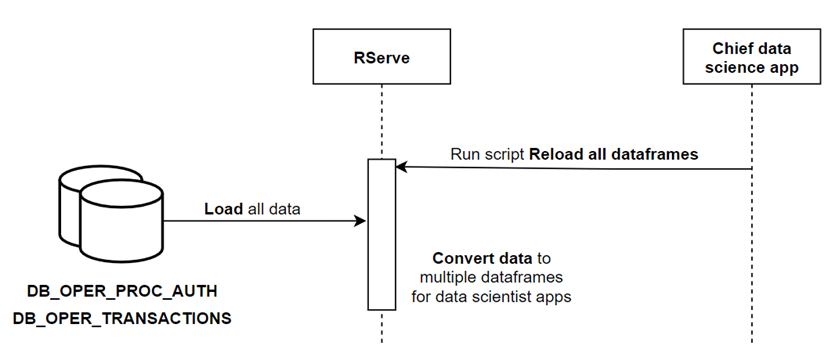
\includegraphics[width=\textwidth]{./img/thibault-Serveur_RServe.png}
    \caption{Échange des données avec l'application Chief}
    \label{fig:thibault-server-rserve}
\end{figure}

\section{Tests}

\subsection{Test de l'API}

Le bon fonctionnement de l'API permettant d'insérer les transactions (NBS) a été testé à l'aide du
framework Cucumber. Cet outil permet de générer des scénarios de texte dans un langage
compréhensible par tout le monde et de relier cette documentation à des fonction java permettant de
tester ces même scénarios (et ainsi, assurer la véracité du scénario). On se retrouve alors avec une
documentation vivante du projet.

En l'occurrence, voici les scénarios qui ont été testés\footnote{Le langage utilisé ci-dessus est appelé Gherkin, et est composé de 'Given' - 'When' - 'Then'. Chacune
de ces lignes est reliée à une fonction qui sera exécuté lors du test du scénario.} :

\begin{figure}[H]
    \centering
    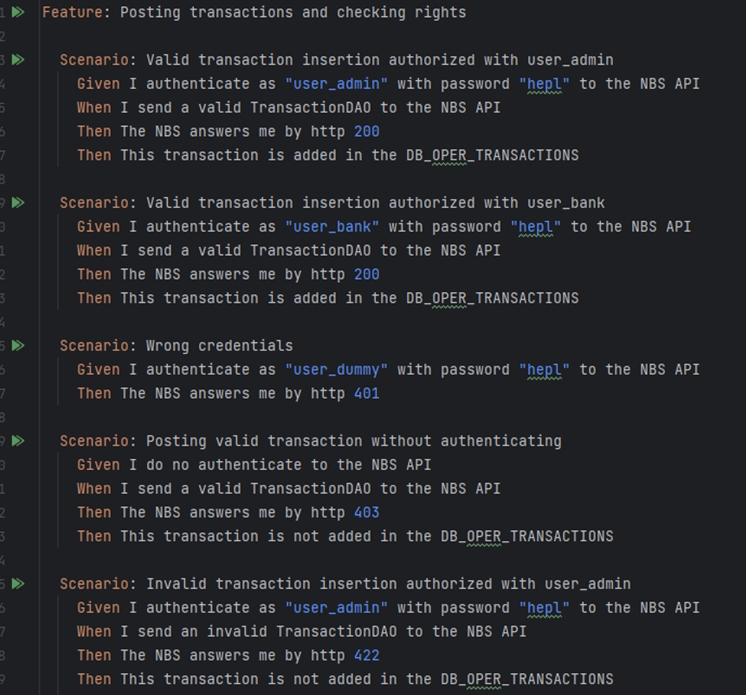
\includegraphics[width=\textwidth]{./img/thibault-Tests_1.png}
    \caption{Représentation des tests unitaires}
    \label{fig:thibault-unit-testing-01}
\end{figure}

Le lien est effectué dans le code à l'aide d'une annotation placée juste avant la définition de la
fonction :

\begin{figure}[H]
    \centering
    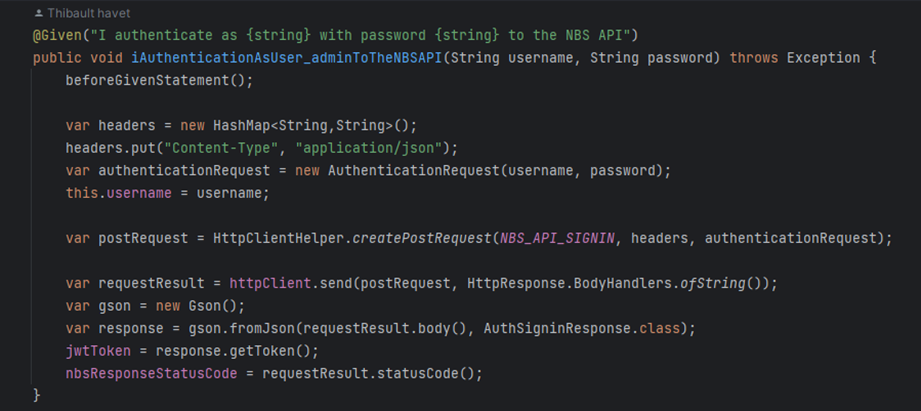
\includegraphics[width=\textwidth]{./img/thibault-Tests_2.png}
    \caption{Code d'un test unitaire en Java}
    \label{fig:thibault-unit-testing-02}
\end{figure}

\subsection{Génération de données bruitées}

Le test de la partie DB\_OPER\_XXX <-> RServe <-> data-scientist-app repose sur un code de génération de données contenu dans le National Bank Server. Cette application a pour but de remplir les 2 bases de données 'DB\_OPER\_XXX' avec des données factices.

Cependant, ces données ne peuvent pas simplement être générée aléatoirement, et il a fallu implémenter plusieurs outils permettant de générer un bruit gaussien (voir le package be.masi\_liege\_g2\_2223.data\_generation.randomizer du projet national-bank-server).

La major partie de ces outils reposent sur un générateur de nombre aléatoire avec une fonction de répartition gaussienne. Par exemple, si l'on souhaite générer un nombre dans un certain intervalle défini par une borne min et une borne max, le calcul est le suivant :

\begin{listing}[H]
    \begin{minted}{java}
// …
do{
    result = Math.round(mean + calculateNoise());
} while(result < min || result > max);
// …

private double calculateNoise(){
    return stdDev * random.nextGaussian();
}
    \end{minted}
    \caption{Génération d'une borne min-max dans un interval}
    \label{listing:thibault-gen-noise}
\end{listing}

Avec 'random' un java.util.Random qui a été initialisé avec 'new Date().getTime()' et la fonction nextGaussian qui renvoie un flottant à double précision aléatoire généré par une Gaussien de moyenne 0 et de variance 1. Afin de pouvoir modifier l'écart type et la moyenne de cette fonction random.nextGaussian(), on multiplie le résultat par l'écart-type voulu (stdDev) et lui ajoute la moyenne voulue (mean).

Une fois ces outils mis en place, il fut aisé de générer les données (voir la classe be.mas\_liege\_g2\_2223.applications.DataGeneration ainsi \\ que le package be.masi\_liege\_g2\_2223.data\_generation du projet national-bank-server).

\subsubsection{Exemple}

On génère des données comme suit du côté du National Bank Server :

\begin{listing}[H]
    \begin{minted}{r}
// -----------------------------
// HOMME de 45 à 75 ans
// -----------------------------
// +EID
// +EMail
// temps auth =~ 25 000ms
// 2 banques
// -----------------------------
// FEMME de 45 à 75 ans
// -----------------------------
// +EID
// +OTP
// temps auth =~ 20 000ms
// 2 banques
// -----------------------------
// HOMME de 20 à 40 ans
// -----------------------------
// +EMail
// +SMS
// temps auth =~ 10 000ms
// 1 banque
// -----------------------------
// FEMME de 20 à 40 ans
// -----------------------------
// +EMail
// +SMS
// temps auth =~ 10 000ms
// 1 banque
    \end{minted}
    \caption{Génération d'une borne min-max dans un interval}
    \label{listing:thibault-generated-data-scheme}
\end{listing}

Ci-dessus, '+Email' signifie que la personne s'authentifie beaucoup plus souvent par Email. En
l'occurrence, '+Email' signifie que sur 260 authentifications, la personne s'authentifiera en moyenne
100 fois par Email (fonction de répartition Gaussienne avec une moyenne de 100 et un écart-type de
20).

On génère :

\begin{itemize}
    \item 150 femmes de 20 à 40 ans
    \item 150 hommes de 20 à 40 ans
    \item 100 femmes de 45 à 75 ans
    \item 100 hommes de 45 à 75 ans
\end{itemize}

Une fois injectée dans des 2 bases de données et passées au serveur RServe, on peut vérifier que les données reflètent ce qui a été établit plus haut. Ici, le serveur RServe a créé un dataframe nommée 'nbrAuthDf' qui permet d'étudier les préférences d'authentification d'une personne. Elle est composée des colonnes suivantes :

NbreBanque - Genre - Age - NbrEID - NbrEmail - NbrOTP - NbrSMS

Après avoir récupéré les données sur l'application du data-scientist (via le serveur RServe) on commence par faire une ACP afin d'établir des corrélations entre des variables quantitatives (elles le sont toute, excepté le genre).

\begin{figure}[H]
    \centering
    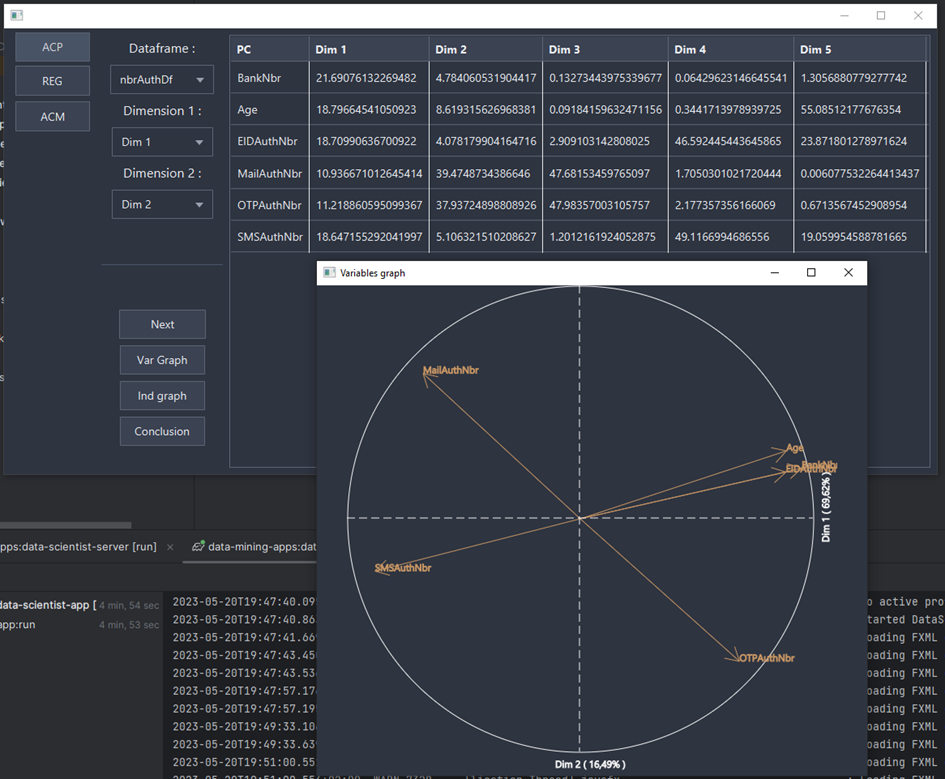
\includegraphics[width=\textwidth]{./img/thibault-Tests_Exemple_1.png}
    \caption{ACP de variables quantitaives}
    \label{fig:thibault-ex-01}
\end{figure}

On constate que la dimension 1 prend énormément d'inertie (69,62\% de l'inertie totale), elle est donc
significative, et permet de mettre en exergue beaucoup d'informations.

De plus, toutes les variables sont bien projetées (loin du centre du cercle).

On observe que l'age, le nombre d'authentification EID et le nombre de banque sont fortement
corrélées. De plus, le nombre d'authentification par SMS et le nombre d'authentification par EID sont
corrélées négativement. Il en va de même avec l'authentification par Mail et avec OTP. De fait, dans les
données générées plus haut, quel que soit la catégorie (jeune/âgé homme/femme), personne ne
s'authentifie souvent par mail ET par OTP (il en va de même pour SMS et EID).

De ce graphique, on en tire également la conclusion que les variables 'Age', 'EIDAuthNbr', 'BankNbr' et
'SMSAuthNbr' (négativement) contribuent fortement à la dimension 1. Par conséquent, les personnes ayant un X positif sur le graphique des individus auront tendance à être plus âgé, à avoir 2 banques, et
à s'authentifier par EID, ou par OTP qui contribue lui aussi, mais un peu moins, à la dimension.

Cependant, s'ils ont un X négatif, ils auront plutôt tendance à être jeunes et à utiliser l'authentification
par mail et SMS.

On retrouve donc bien les caractéristiques établies dans les données factices.

Petite parenthèse sur la variable 'Email' : celle-ci se situe plus à gauche, alors que certaines personnes
âgées l'utilisent également. De fait, il y a 300 jeunes qui ont été généré, pour seulement 200 personnes
plus âgées, et seules 100 personnes l'utilisent.

Passons maintenant à la régression-corrélation multiple. On commence par une régression à une variables explicative. On va tenter d'expliquer la variable 'SMSAuthNbr' par l'age :

\begin{figure}[H]
    \centering
    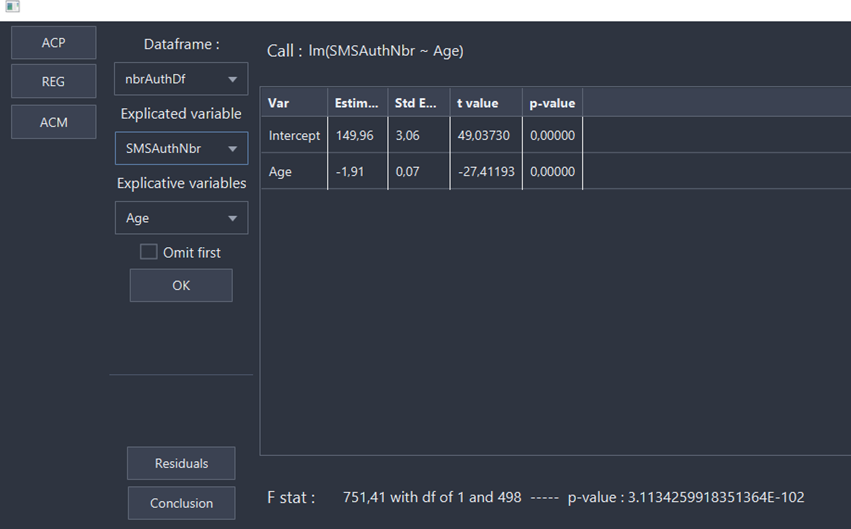
\includegraphics[width=\textwidth]{./img/thibault-Tests_Exemple_2.png}
    \caption{p-values de Fischer}
    \label{fig:thibault-ex-02}
\end{figure}

On constate que le modèle est fiable (p-value de Fisher avec vraiment infime) et le paramètre 'Age'
du modèle est également très fiable (p-value de 0).

Un petit peu plus compliqué maintenant, on va tenter d'expliquer la variable 'SMSAuthNbr' en
fonction des 3 variables qui lui sont corrélées négativement :

\begin{figure}[H]
    \centering
    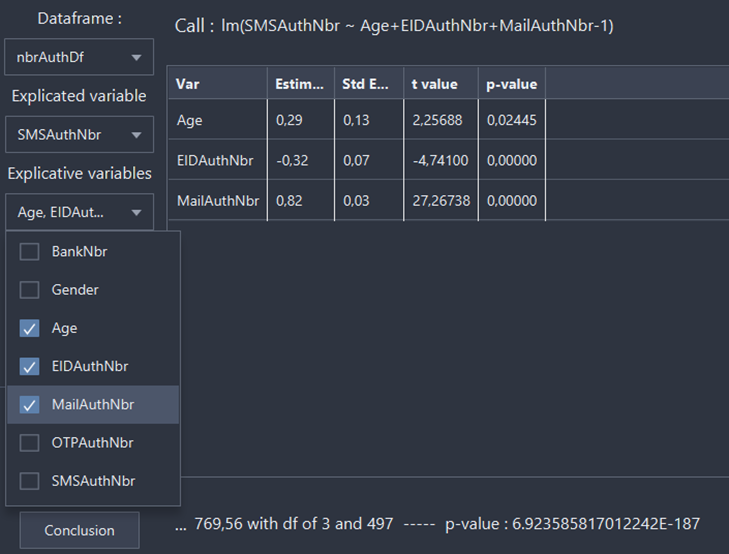
\includegraphics[width=\textwidth]{./img/thibault-Tests_Exemple_3.png}
    \caption{p-values de Fischer}
    \label{fig:thibault-ex-03}
\end{figure}

On obtient une p-value de Fisher encore plus petite. Les coefficient 'Age', 'EIDAuthNbr'et
'MailAuthNbr'sont également très fiable (p-value valant 0 ou en étant proche).

Il n'est ici pas possible de réaliser une ACM en raison du nombre de variables qualitative. Pour ce
faire, il faut s'en référer à un autre jeu de données :

\begin{listing}[H]
    \begin{minted}{r}
// -----------------------------
    // HOMME AGE
    // -----------------------------
    // +EID
    // +EMail
    // +Capricioso
    // +Du chef
    // 60% de personnes divorcées - 30% marriées
    // + delMolin et +Andrea
    // -----------------------------
    // FEMME AGEE
    // -----------------------------
    // +OTP
    // +Mezzo mezzo
    // +Du chef
    // 60% de personnes divorcées - 30% marriées
    // + pinocchio et +Andrea
    // -----------------------------
    // YOUNG PEOPLE
    // -----------------------------
    // +SMS
    // +Margerita
    // +Calzone
    // 40% de single - 30% married - 20% divorced
    // +pizza hut
    \end{minted}
    \caption{Génération d'une borne min-max dans un interval}
    \label{listing:thibault-another-data-set}
\end{listing}

Même procédé que le précédent (100 personnes plus âgées de chaque sexe, et 300 jeunes). Le
serveur RServe transforme ces données en la dataframe suivantes :

"Amount", "Account Previous State", "Merchant", "Gender", "Age", "Marital Status", "Monthly
Salary", "Auth type", "Product" (la variables product est ici composées de pizza).

On supprime donc toutes les colonnes quantitatives, on se retrouve alors avec les colonnes
suivantes : "Merchant", "Gender", "Marital Status", "Auth type", "Product"

On effectue ensuite l'ACM et on en étudie les valeurs propres :

\begin{figure}[H]
    \centering
    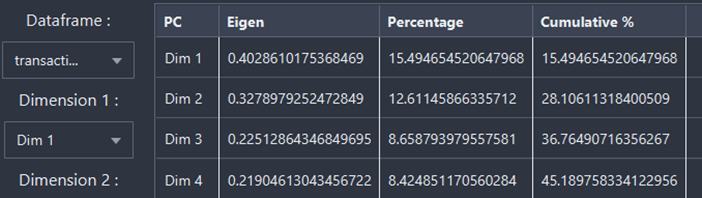
\includegraphics[width=\textwidth]{./img/thibault-Tests_Exemple_4.png}
    \caption{Résultat de l'ACM}
    \label{fig:thibault-ex-04}
\end{figure}

Les 2 premières dimensions sont plutôt convaincantes, prenant 28\% de l'inertie totale, ce qui n'est
pas rien pour une ACM (puisque l'inertie est diluée dans les modalités rajoutées).

\begin{figure}[H]
    \centering
    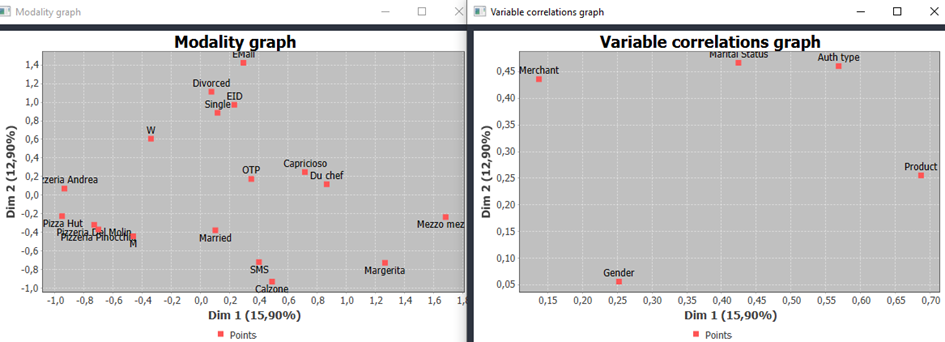
\includegraphics[width=\textwidth]{./img/thibault-Tests_Exemple_5.png}
    \caption{Les carrés des corrélations et le graphique des modalités (pour la dim. 1 et 2)}
    \label{fig:thibault-ex-05}
\end{figure}

On observe par exemple que les personnes qui s'authentifient par SMS mangent des calzone (lesau
jeunes), que les personnes qui mangent des pizzas 'Du chef' consomment également des pizzas
'Capricioso' (les homes plus âgés).

Cependant, on remarque quelques incohérences comme les personnes qui utilisent EID qui ont
tendances à être divorcées ou célibataire. Pareil pour les marchants qui sont tous collés les uns aux
autres.

\subsection{A refaire}

La réalisation de cette partie du projet intégrée fut beaucoup trop longue, le développement de la
branche data-scientist (NBS + DSS ainsi que les 2 applications et la gestion des 4 bases de données) a
pris plus de 60h de développement. Si cela était à refaire :

\begin{itemize}
    \item Nous n'aurions pas utilisé Rserve. De fait, cette librairie souffre de 2 défauts majeurs :
    \begin{itemize}
        \item Le débogage est inexistant. De plus, quel que soit l'erreur commise lors de l'exécution d'une commande depuis java, le serveur envoie le code d'erreur 127 sans aucun autre message.
        \item La récupération des données depuis R vers java (et inversement) est un travail d'orfèvre. En effet, il faut appeler une méthode par champs à récupérer, ce qui peut mener à des fonctions gargantuesque au code immonde (voir la classe be.masi.g2.
        REngineRServeUtils.Utils.RDataMediator).
    \end{itemize}
    \item Nous aurions utilisé les interfaces de REngine pour afficher les résultats. En l'état des choses,
    tous les résultats des méthodes d'exploration de données (ACP, régression linéaire multiple,
    ACM) sont extraits de R, convertit en un objet java et ensuite affiché dans une fenêtre JavaFX
    (en utilisant la librairie JFreeChart ou non).
    Cependant, la conception de chacune de ces fenêtres nous a pris beaucoup trop de temps.

    \textbf{NB} : En réalité, il aurait été plus judicieux d'utiliser des notebooks. De fait, ceux-ci présentent
une plus grande flexibilité (le data-scientist peut écrire lui-même le code et utiliser les
méthodes qu'il désire, sans devoir passer par une nouvelle fenêtre JavaFX pour chaque
afficage). Une fois la conclusion tirée, le Data-Science-Server aurait stocké le notebook dans la
DB\_DECIS\_TEMP, etc, etc.

    \item Nous aurions optimisé le menu de l'application data-scientist. De fait, la fenêtre de démarrage
    charge toutes les informations de chacune des conclusions, ce qui n'est pas optimisé. Il aurait
    fallu charger les informations strictement nécessaires telles que le titre de la conclusion,
    l'auteur, la date de la conclusion, …
\end{itemize}


\Chapter{Module d'authentification par carte d'identité et gestion de points de fidélité par smartcard}{Andrea Dal Molin}

\section{La Belgian eID}

La carte d'identité électronique belge est entrée en vigueur en 2004. Elle comporte une carte à puce qui contient plusieurs informations quand au propriétaire de la carte. Elle permet au citoyen de s'authentifier mais également, pour les majeurs, de signer des documents. Elle comporte donc deux certificats: une d'authentification et un de signature (uniquement le premier pour les moins de dix-huit ans).

\subsection{But et fonctionnement}

Le but de l'intégration des eID au sein du projet est celui de permettre à l'utilisateur qui paie sur un site marchand de s'authentifier auprès de sa banque pour confirmer et valider le paiement. Pour faire cela il devra passer par les étapes suivantes: 

\begin{itemize}
    \item Entrer sa carte dans un lecteur de cartes
    \item Ouvrir l'application d'authentification eID
    \item Entrer son numéro de client après de la banque et le PIN de sa carte de crédit 
    \item  Signer avec son PIN de l'eID 
\end{itemize}

Par la suite de ces étapes, si toutes les informations sont correctes, le banque aura toutes les informations pour valider et donc autoriser le paiement. 

\subsection{Implémentation du module}

Le module d'authentification a été codé sous la forme d'une application Java, plus précisément utilisant
le JDK 19. Cette application client s'affiche au client grâce à une interface crée avec JavaFX. Le module
gère tout ce qui concerne la lecture de la carte elle-même mais également les échanges avec la
banque. Ces-derniers sont sécurisés via un chiffrement symétrique qui fonctionne via l'utilisation
d'une clé de session sur des Socket.
Le programme nécessite l'installation d'une DLL, nommée beidpkcs11.dll qui permet de s'interfacer et
de communiquer avec la carte. Cette DLL s'installe automatiquement lors de l'installation de
l'eIDViewer\footnote{https://eid.belgium.be/en}, un logiciel fourni par le Gouvernement Belge. Il est également nécessaire d'utiliser le
standard PKCS11, un protocole de cryptographie à clé publique. Dans notre cas, nous avons utilisé un
fichier de configuration standard fourni par les professeurs. Bien-sûr il faut également être en
possession d'un lecteur de carte, qui permettra de lire l'eID.
Une fois ce prérequis remplis, le client Java a tout ce dont il nécessite pour fonctionner.

\subsection{Fonctionnement pratique}

Il est évident que les échanges entre le Client et la Banque doivent être sécurisés, car les informations
qui transitent sur ces messages sont des données sensibles. Pour ces raisons, nous avons réfléchis à
un système qui permette d'assurer cette sécurité. Le diagramme qui suit illustre les premiers échanges
entre le Client, la Banque et le serveur de certificats.

\begin{figure}[H]
    \centering
    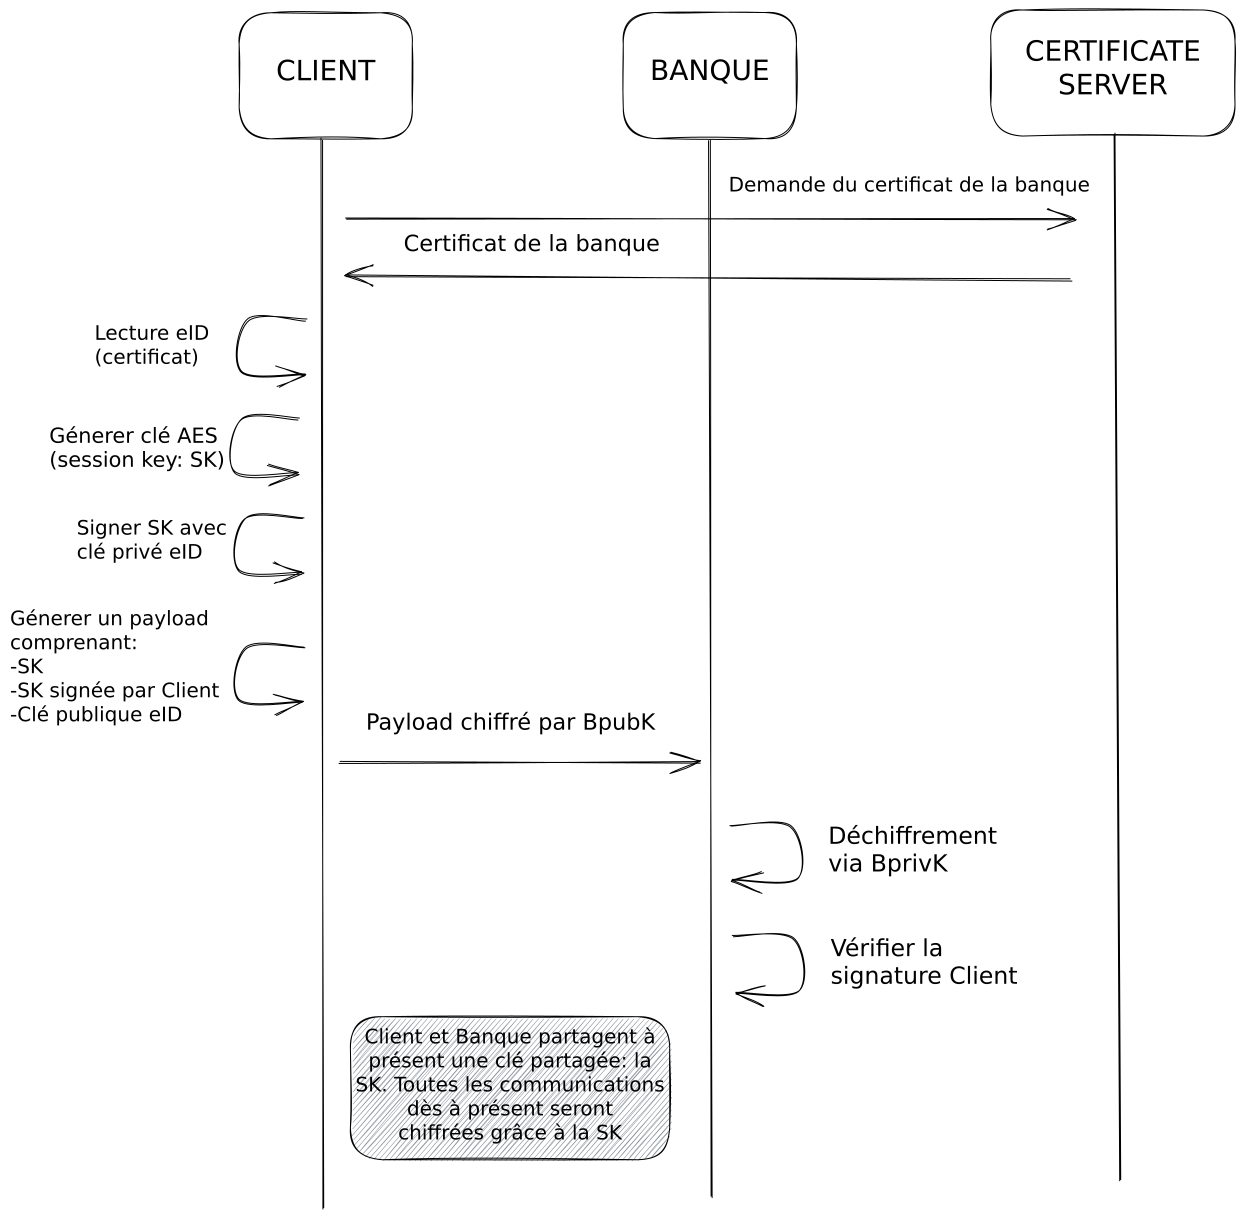
\includegraphics[width=\textwidth]{img/andrea-fig-1.png}
    \caption{Premiers échanges entre Client, Banque et Serveur de certificats}
    \label{fig:smartcard-exchange}
\end{figure}

Premièrement, le Client possède son certificat extrait de l'eID. Ceci lui donne accès à la clé publique
de son certificat, et à la clé publique. Cependant cette dernière n'est utilisable que pour la signature
de messages, et non pas pour chiffrer.
Nous constatons que les premiers échanges concernent le partage des clé publiques, et le plus
important, la création d'une clé de session. Celle-ci nous permettra de chiffrer les futurs échanges
entre Client et Banque. La clé de session (\textbf{SK}) est générée du côté du Client, qui s'occupe également de la signer, pour prouver son authenticité à la banque. De plus il envoie également sa clé publique à
la Banque, pour que celle-ci puisse vérifier cette signature. Ces trois blocs d'information sont envoyés
en un seul message chiffré avec la clé publique de la Banque. Ceci signifie que seule la Banque pourra
le déchiffrer.

Dès à présent, tous les futurs messages seront chiffrés via la clé de session, qui a été échangée entre
Client et Banque de manière sécurisée. Maintenant débute la véritable vérification qui autorisera le
paiement.

\begin{figure}[H]
    \centering
    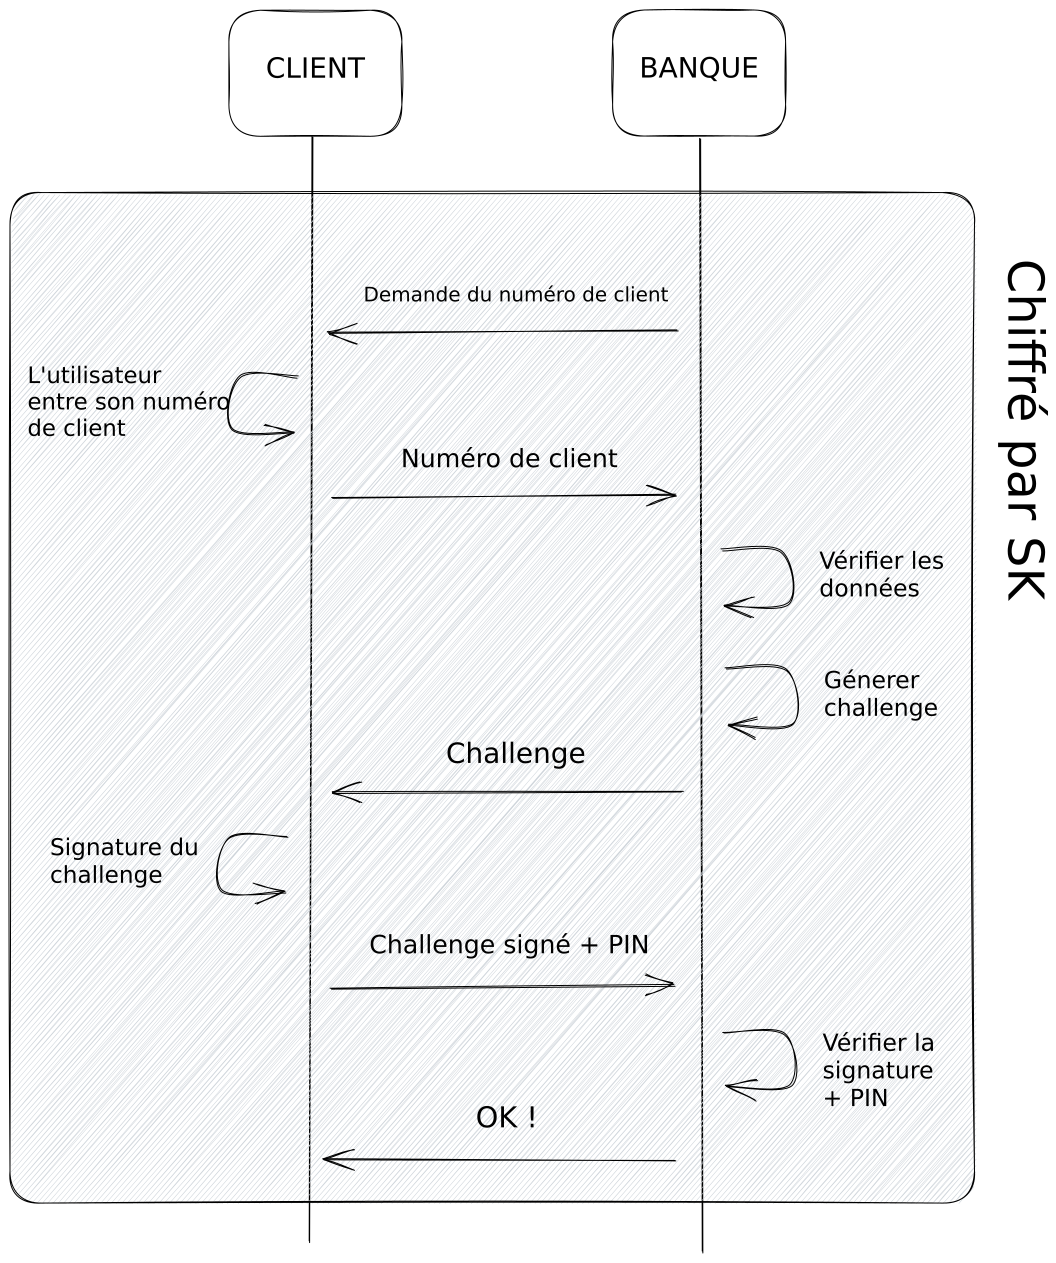
\includegraphics[scale=.5]{img/andrea-fig-2.png}
    \caption{Seconde phase de l'authentification}
    \label{fig:smartcard-exchange02}
\end{figure}

En cette seconde phase, nous traitons les données plus sensibles, d'où la nécessité du chiffrement
garanti par notre clé de session. Une fois que la banque reçoit le numéro de client demandant
autorisation, elle générera un challenge, qui sera signé par le client. Lorsque cette signature est
vérifiée, le paiement est autorisé et l'échange se termine.

\section{Gestion de points de fidélité par smartcard}

Pour cette tâche, nous avons utilisé la technologie Java Card, présentée au cours de Smartphone et
Cartes à Puces. Pour des raisons de simplicité, de respect de l'environnement et de limitations
d'infrastructure, nous nous sommes limités à l'utilisation d'un simulateur de Java Card plutôt
qu'investir dans du réel matériel dont l'utilisation future pourrait n'être que fortement limitée.
Les points de fidélité trouvent confortablement leur place au sein du projet intégré dans le cadre d'une
gamification de l'expérience d'achat, qui, dans un cas plus développé du projet, pourrait donner la
possibilité à l'acheteur de bénéficier de réductions et avantages.

\subsection{But et fonctionnement}

Le cartes de fidélité fonctionnent de paire avec les sites et bases de données marchandes. Ces
dernières gardent une traces des achats d'un client. Sur base de ses achats, il accumulera un certain
nombre de points. Ces points sont calculés automatiquement du côté des marchands. Le cartes de
fidélité entrent en jeu lors des achats faits physiquement en magasin. Par exemple, lors d'une
promotion spéciale, le client a droit à 50\% plus de points pour ses achats en magasin. Ceci est géré
donc par la petite application crée pour ce projet. L'utilisateur, qui sera de fait le responsable de caisse
ou autre travailleur du marchand, scannera la carte de fidélité et aura la possibilité d'ajouter un certain
nombre de points pour le client. Un autre cas pourrait être l'échange des points pour une réductions
sur le total des achats. Dans ce cas, le responsable pourra aussi soustraire des points de la carte. Toutes
ces manipulations sont reflétées dans la base de données qui sera notifié et mise à jour à chaque
changement sur la carte.

\subsection{Fonctionnement du module}

Concrètement, l'application est matérialisée par une application Java, qui fonctionne en mode console.
L'absence d'une interface graphique a été due à des difficultés rencontrés à cause d'une incompatibilité
entre la version de Java nécessaires au bon fonctionnement de certaines librairies qui s'interfacent
avec les cartes Java Card. Le module est séparé en deux parties.
La première, qui constitue le cœur de la Java Card est l'applet. Cette partie a été codée sur la version
7 de Java et en utilisant le JCDK (Java Card Development Kit). L'applet défini la véritable structure de la
carte et défini non seulement les données qu'elle contiendra mais également les opérations que celle-
ci peut opérer. Dans notre cas, nous stockons simplement deux informations sur la carte : un identifiant
du propriétaire et le total de ses points. A côté de cela, les opérations qui sont stockées sur la carte
concernent la lecture et l'écriture de ces variables. D'autres méthodes supplémentaires permettent de remettre à zéro les total des points, de réattribuer le propriétaire de la carte et de reset la carte
totalement. Cette applet est donc compilée grâce au JCDK (Java Card Development Kit) et écrit dans la
mémoire EEPROM de la carte à puce.

\begin{listing}[H]
    \begin{minted}{java}
        public class AppletProjetIntegre extends Applet {
            /******************* Constantes ****************/
            public static final byte CLA_PROJECTAPPLET = (byte) 0xB0;
            public static final byte INS_GET_POINTS = 0x00;
            public static final byte INS_SET_POINTS = 0x01;
            public static final byte INS_RES_POINTS = 0x02;
            public static final byte INS_GET_ID = 0x03;
            public static final byte INS_SET_ID = 0x04;
            public static final byte INS_RES_ID = 0x05;
            public static final byte INS_RES_CARD = 0x06;
        
            /**************** Variables *******************/
            private byte id;
            private byte points;

            private AppletProjetIntegre() {
                id = 0;
                points = 0;
            }

            /*
                ...
            */
        }
    \end{minted}
    \caption{Définition des variables et des fonctions présentes sur la Java Card}
    \label{listing:applet-projet-integre}
\end{listing}

La seconde partie du client est le programme qui s'interface à la carte et l'interroge. Les méthodes
définies dans l'applet via des codes hexadécimaux sont réutilisées dans ce même projet, qui utilise les
codes pour échanger des informations avec la carte. Ici est également cachée la logique qui appelle
l'API du marchand.
Dès l'insertion de la carte, le programme vérifie d'abord qu'un identifiant est bien présent sur la carte.
Le cas échéant, le programme demande d'attribuer la carte à quelqu'un. Le responsable dans ce cas
entre le nom ou l'email du client, et, si celui-ci est enregistré dans la base de données du marchand, la
carte est initialisée avec les l'identifiant du nouveau propriétaire et ses points actuels sont également
écrits. Une fois la carte prête, le responsable a la possibilité d'ajouter, de soustraire ou de simplement
consulter le nombre de points disponibles sur la carte.

\section{Conclusions personelles}

Du point de vue personnel, ce projet fut un grand défi, tant du point de vue technique, que de celui
d'organisation. Le déroulement du projet s'est bien passé grâce à une bonne ambiance et une bonne
entente au sein du groupe.
Du point de vue technique, la partie eID a sans doute été le plus grand défi. L'absence de réelle
documentation ont rendu le développement d'autant plus lent et souvent basé sur du « trial and
error ». Cependant cela a résulté en une bonne compréhension du fonctionnement des carte
d'identité électroniques et sur les possibilités qu'elles offrent. La partie Java Card, s'est déroulé avec
moins de difficultés, du moins pour la programmation de l'applet.
Du point de vue de l'organisation, la plus grande difficulté rencontré a été celle de l'organisation du
travail au sein de l'équipe et la répartition des tâches. Nous avions initialement pensé que la partie eID
et Java Card était plutôt isolé du reste du projet et cela est vrai, mais uniquement partiellement. J'ai
personnellement dû me coordonner avec d'autre membres du groupe pour compléter des parties de
mon travail, et j'ai essayé d'aider quand cela m'était possible.
Globalement, j'estime que nous avons tous beaucoup appris sur les projets en équipe, sur les difficultés
qu'ils présentent et sur la manière de les affronter. Si nous devions recommencer le projet, nous
porterions sans doute une attention plus importante quant à la définition plus précise de sprint et à la
répartition des tâches, qui dans le cas de notre groupe a parfois été sous-optimale


\Chapter{Testing et assurance qualité des produits}{Alexandre Villance \& Flo Raeymaeckers}

\input{chapters/08-testing.tex}

\Chapter{Gestion de l'équipe}{Flo Raeymaeckers}

La gestion d'équipe, ça n'est pas un tâche facile. La gestion du projet en parallèle, encore moins. Et le déploiement de l'ensemble des systèmes mis en place par l'équipe, plus qu'un challenge.

\section{Agile \& SCRUM}

La méthodologie de travail que nous avons choisi d'adopter s'inspire de la méthodologie Agile et des principes SCRUM. L'Agile a clairement ses avantages par rapport à d'autres méthodologies de travail. Cependant, les restrictions suivantes a rendu notre méthodologie moins "agile" que l'on aurait espérer:

\begin{itemize}
    \item La contrainte du temps: le projet devait être développer sous 3-4 mois. La méthodologie Agile permet le suivi d'un projet plus efficace et avec un rendement amélioré, au détriment du temps, cependant. Cela veut dire que nous prenons plus de temps à mettre en place le projet pour que ce dernier soit qualitatif et que le suivi de ce dernier soit aisé. Malheureusement, le principe de manque de temps sera le leitmotiv récurrent de ce rapport.
    \item La contrainte de l'école: un peu liée avec la contrainte précédente, le fait que l'on soit à l'école restreint certaines choses. Premièrement, nous devons travailler pour d'autre cours en parallèle, ce qui ralenti encore plus le développement. Ensuite, un des principes agiles est de faire une réunion quotidienne (et matinale) d'une dizaine de minutes afin de receuillir l'avancement de chacun. A la place d'une réunion quotidienne, nous avons opté pour une réunion hebdomadaire, mais cela ne valait pas une réunion quotidienne.
\end{itemize}

Ce genre de méthodologie requiert aussi une grande analyse du projet à l'avance, ce qui a été compliqué au départ. J'ai moi-même voulu commencer à travailler ce projet assez tôt, mais l'énoncé de ce dernier nous a été parvenu qu'un mois après mon pic de motivation. De plus, l'énoncé a été une part de difficulté dans notre façon de faire car nous avions dû déchiffrer certaines parties, et cela nous a pris pas mal de temps.

\section{YouTrack: notre outil de gestion de projet}

Afin de gérer les différentes deadlines et les tâches assignées à certains projets, j'ai décidé de partir sur un hébergement sur le cloud d'une version gratuite de YouTrack.

\begin{figure}[H]
    \centering
    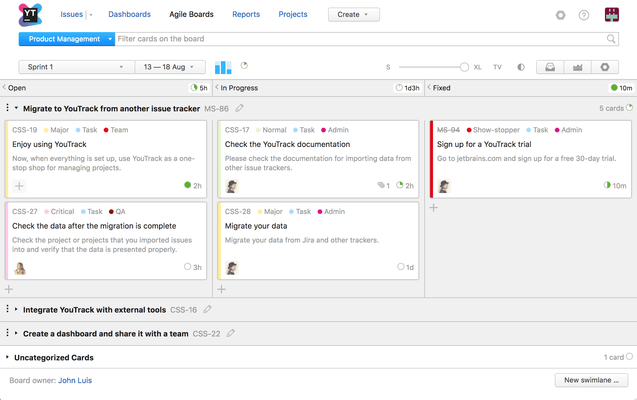
\includegraphics[width=\textwidth]{./img/youtrack.png}
    \caption{Exemple de l'interface de YouTrack (non représentatif de notre projet)}
    \label{fig:youtrack}
\end{figure}

La customisation et la classification des différentes tâches est totalement customisable par l'administrateur de YouTrack (c'est-à-dire moi). Ensuite, les utilisateurs vont pouvoir créer leur tâches en leur assignant un projet, l'importance de la tâche, le temps passé dessus, le temps estimé\dots enfin bref, quelques paramètres bien sympatique au suivi du projet. De plus, il y avait moyen d'afficher un Gantt Chart, ce qui permettait de voir l'avancée du projet et les différentes deadlines des tâches.

\begin{figure}[H]
    \centering
    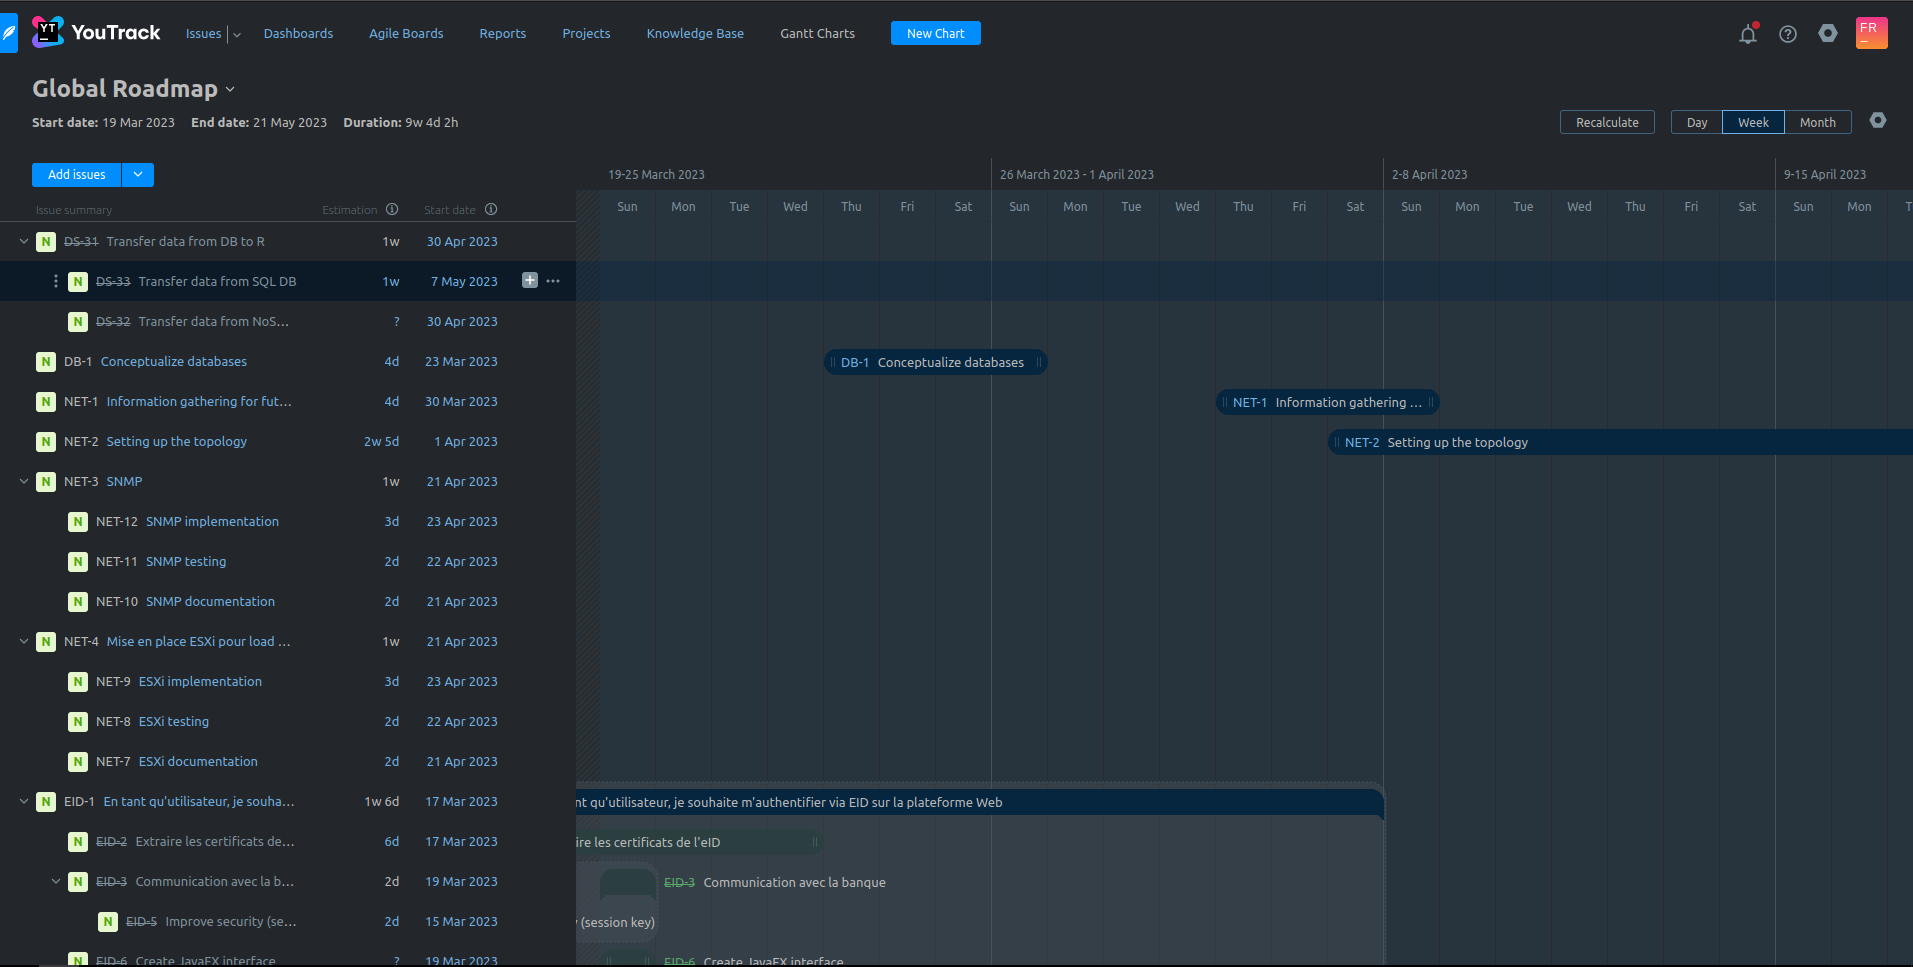
\includegraphics[width=\textwidth]{./img/youtrack-gantt.png}
    \caption{Vue du projet sous un graphe de Gantt}
    \label{fig:youtrack-gantt}
\end{figure}

\section{Difficultées encourrues}

\subsection{L'organisation des rôles}

L'une des premières difficulté qu'on a rencontré en tant qu'équipe est la réassignation des rôles. Étant une équipe avec moins de pairs qu'estimé initialement (8 à la place de 9), certains rôles n'étaient pas assignables. Joignez à ça la vague idée que l'on avait du projet au début, et ça nous compliquait l'assignation des rôles. Finalement, nous nous étions mis d'accord sur un tableau de rôles.

\begin{figure}[H]
    \centering
    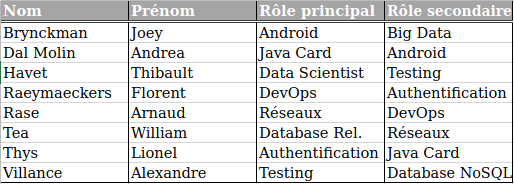
\includegraphics[width=\textwidth]{./img/roles.png}
    \caption{Tableau des rôles rendu au professeur responsable}
    \label{fig:roles}
\end{figure}

En tant qu'étudiante bachelière ayant suivi une formation de développement d'applications, ce principe de rôle m'eût parut bizarre. De fait, si cette contrainte n'était pas à rendre si tôt ni même existante, je pense que j'aurais: soit annuler toute notion de "rôle", et de naturellement laisser les personnes se diriger vers ce qui leur plaît (certains aurait peut-être préféré développer que de faire du réseau, par exemple), soit assigner les rôles après avoir analyser les différentes parties du projet (même si je préfère clairement la première approche). L'avantage aussi de cette première approche est que, si quelqu'un bloque sur une tâche, un autre pourra se permettre de l'aider ou bien de reprendre sa tâche et de tout de même avancer, surtout si c'est une tâche critique.

Un autre gros soucis avec la méthodologie des rôles, est que, vers la fin du projet, nous nous sommes retrouvé avec certains qui avait moins contribué que d'autres car leur rôle n'avait aucun sens comparé aux autres. La charge des différents rôles était déjà difficilement estimable, mais en plus nous nous sommes rendus compte de l'inégalité de ladite charge.

\subsection{Préparation \& Analyse du projet}

L'analyse de l'énoncé du projet était une étape fastidieuse. Premièrement, on ne savait pas réellement où donner de la tête. Là où certains avait beaucoup à analyser à cause de leur rôle (i.e. Joey et la conception de l'applcation mobile), d'autre n'avaient pas réellement beaucoup à faire car une analyse n'était pas vraiment nécessaire (i.e. les bases de données relationnelles). Cette étape était très importante car il eut fallu, au final, transformer cet énoncé en User Stories à encoder dans l'outil de gestion de projet. Malheureusement, même si nous avons eu en globalité quelques User Stories intéressantes, l'utilisation de ces dernières n'a pas été au plus efficace.

\subsection{Le testing}

Si vous avez l'oeil, vous aurez remarqué que nous ne parlons pas énormément du testing. Autant certain l'ont appliqué localement, c'est-à-dire qu'ils ont mis en place des tests unitaires. Autant, globalement, ça n'était pas supervisé ni même encouragé. Et, ça été plus un manque de gestion général que le problème de la personne responsable du testing. Le but était le suivant: Analyser l'application, mettre en place des User Stories, faire des tests basés sur ces User Stories et puis enfin implémenter la solution. Cependant, c'est premièrement quelque chose qui, comme pour la méthodologie agile, demande plus de temps qu'initalement car nous avons besoin de mettre en place tout les tests derrière avant le commencement du développement. Encore une fois quelque chose qui demande du temps.

Je suis une des premières à dire que le testing est une étape très importante dans le développement et la mise en place d'une solution logicielle. Cependant, qu'aurions nous fait si, à la finalité du projet, nous aurions tous les tests soigneusement écrits, mais aucune implémentation concrète de la solution de l'énoncé ?



\chapter{Améliorations du projet}

\input{chapters/10-improvement.tex}

\section{Niveau de l'exécution du projet}

\section{Niveau de la gestion d'équipe}

\bibliographystyle{plain}
\bibliography{ref}

\end{document}
